\documentclass[10pt,journal,compsoc]{IEEEtran}
\IEEEoverridecommandlockouts
\usepackage{cite}
\usepackage{amsmath,amssymb,amsfonts}
\usepackage{algorithm}
\usepackage{algorithmic}
\usepackage{graphicx}
\usepackage{textcomp}
\usepackage{xcolor}
\usepackage{booktabs}
\usepackage{multirow}
\usepackage{array}
\usepackage{pgfplots}
\pgfplotsset{compat=1.17}
\usetikzlibrary{positioning,arrows.meta,fit,backgrounds,shapes.geometric}

\usepackage{url}

\begin{document}

\title{SEVA: Characterizing and Delimiting Cohesion-Based
Detection of Corpus Poisoning in Retrieval-Augmented Generation\\[2pt]
\large\normalfont(Extended Version)}

\author{\IEEEauthorblockN{Anonymous Author(s)}
\IEEEauthorblockA{Manuscript submitted for blind review}}

\maketitle

\begin{abstract}
Retrieval-Augmented Generation (RAG) systems are vulnerable to corpus
poisoning---adversarial document injection that corrupts retrieval without
modifying model weights or triggering lexical filters. Existing defenses
require LLM decoder access, multiplicative inference overhead, or cryptographic
pre-registration, making them impractical for the on-device, offline deployment
that local AI increasingly demands. We present SEVA, a fully local, LLM-free
detector built on a single geometric signal---per-document $K$-nearest-neighbour
cluster coherence (\texttt{cluster\_coh})---operated as a hard gate, targeting
templated multi-passage poisoning, the dominant published attack pattern
(PoisonedRAG). In-domain, where clean and poison share the \emph{same} security domain
and a geometric signal has no topic shortcut, SEVA drives templated poison-evasion to
0\% across three seeds---a 95\% Wilson upper bound of 0.0154\% from 25{,}000 templated
encounters at the frozen gate---at a 0.58\% document-level false-positive rate, under
frozen non-oracle calibration and 1--10\% contamination density. On PoisonedRAG's
\emph{own released} poison for the field's general-domain benchmarks (Natural Questions,
HotpotQA), and a faithful black-box build on the in-domain Security corpus, it catches
the attack at 82--98\%, while the lexical duplicate filtering PoisonedRAG itself found
insufficient proves corpus-fragile at matched false-positive rate. End to end the gate prevents
all the corruption it detects: the templated attack corrupts 18\% of targets undefended and 0\%
with the gate in the loop. We then delimit the assumption it rests on. \emph{Host-anchored
cloning}---one benign host mimicked per injected passage---evades the gate on every target while
staying retrievable, no complementary geometric signal we tested closes the gap, and the bypass
is not expensive: it corrupts 26--28\% of targets, more than the templated attack achieves
undefended. Reproducing CleanBase, the closest corpus-level peer, at a matched operating point
yields the same pattern (100\% templated, 0\% clones), so the boundary belongs to the shared
mutual-similarity assumption rather than to our statistic. The signal is \emph{encoder-invariant}---%
templated-poison detection generalizes across three embedding models of independent
lineages, bge (BAAI), e5 (Microsoft), and gte (Alibaba)---and \emph{reproducible to
within $5\times10^{-7}$} across two accelerator backends (CUDA and Apple Silicon) on a
byte-identical, hash-verified corpus, several cells bit-identical. Detection stays flat
to a million documents (sub-millisecond retrieval-plus-gate cost at $10\times$ the primary
corpus, the $O(\log N)$ claim measured, not extrapolated), and SEVA runs in $13$--$38$\,ms
per query with no LLM, API, or pre-registration; in a reproduced, shared-corpus,
matched-FPR head-to-head it catches 100\% of templated poison to the per-query state of
the art's $\sim$89\%, which that baseline reaches only at a false-positive rate that
discards roughly half the clean corpus. SEVA is deliberately scoped to one dominant
attack family---templated multi-passage injection, defended across domains, adaptive
adversaries, encoders, and hardware; single-document injections crafted to mimic the
clean distribution are a separate problem, stated as such.
\end{abstract}

\begin{IEEEkeywords}
Retrieval-Augmented Generation, Corpus Poisoning, Anomaly Detection, Embedding
Security, Geometric Detection, On-Device Security.
\end{IEEEkeywords}

\section{Introduction}

\subsection{Motivation}
\begin{figure}[t]
\centering
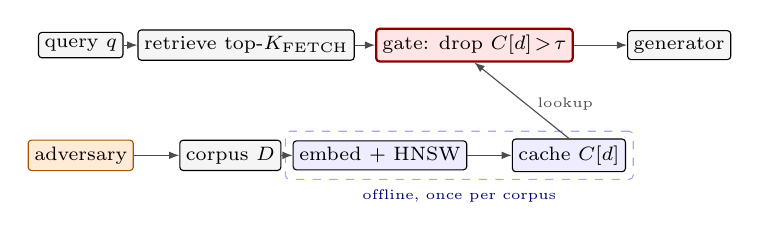
\begin{tikzpicture}[
  font=\scriptsize, x=1mm, y=1mm,
  box/.style={draw, rounded corners=1.2pt, align=center, inner xsep=2.2pt, inner ysep=2.4pt},
  off/.style={box, fill=blue!7},
  on/.style={box, fill=black!4},
  gate/.style={box, fill=red!10, draw=red!55!black, thick},
  adv/.style={box, fill=orange!16, draw=orange!65!black},
  ar/.style={-{Latex[length=1.3mm]}, gray!60!black},
]
% --- online path (top row) ---
\node[on]   (q)   at (0,14)  {query $q$};
\node[on]   (ret) at (21,14) {retrieve top-$K_{\mathrm{FETCH}}$};
\node[gate] (g)   at (50,14) {gate: drop $C[d]\!>\!\tau$};
\node[on]   (gen) at (76,14) {generator};
% --- offline path (bottom row) ---
\node[adv]  (atk) at (0,0)  {adversary};
\node[on]   (cor) at (19,0) {corpus $D$};
\node[off]  (emb) at (38,0) {embed $+$ HNSW};
\node[off]  (coh) at (62,0) {cache $C[d]$};
\draw[ar] (q)   -- (ret);
\draw[ar] (ret) -- (g);
\draw[ar] (g)   -- (gen);
\draw[ar] (atk) -- (cor);
\draw[ar] (cor) -- (emb);
\draw[ar] (emb) -- (coh);
\draw[ar] (coh.north) -- node[right=0.5pt, font=\tiny, pos=0.45] {lookup} (g.south);
\begin{scope}[on background layer]
\node[draw=blue!35, dashed, rounded corners=1.5pt, fit=(emb)(coh), inner sep=2.6pt] (ob) {};
\end{scope}
\node[blue!45!black, font=\tiny, anchor=north] at (ob.south) {offline, once per corpus};
\end{tikzpicture}
\caption{Where the gate sits. The only per-query work SEVA adds is a threshold comparison against
a cached statistic (red); the neighbourhood computation is offline and amortized over every
subsequent query. No LLM is consulted for detection, and the generator is never asked to
adjudicate its own context.}
\label{fig:pipeline}
\end{figure}
Retrieval-Augmented Generation (RAG)~\cite{lewis2020} grounds a language model's
output in an external document corpus, decoupling parametric model knowledge from a
non-parametric, operator-maintained vector store. That decoupling is also RAG's
security liability: it relocates factual authority to a corpus an adversary may
be able to write to. \emph{Corpus poisoning} exploits this. An adversary with
write access to the ingestion pipeline injects crafted documents that are
retrieved at query time and steer the model toward attacker-chosen outputs---%
operating at the infrastructure layer beneath the LLM, without modifying model
weights, and without leaving the lexical traces a keyword filter would catch.

The dominant instantiation is PoisonedRAG~\cite{poisonedrag}, which decomposes
each malicious text into a retrieval-satisfying component and a
generation-satisfying payload and injects five such passages per target
query, reaching 90--97\% attack-success even in corpora of millions of
documents. Two properties of this attack are decisive for the defender. First,
it is \emph{templated}: the passages injected for a target query are generated
from a shared recipe and are therefore mutually similar. Second, it is
\emph{multi-passage}: several co-retrieved passages are injected per query to
dominate the retrieval window. Together they mean the poison enters the corpus
as a tight \emph{cluster} of mutually similar documents---a geometric signature
intrinsic to the attack's own mechanism, and, as we show, present regardless of
how much of the corpus is poisoned.

\subsection{The Deployability Gap and Our Approach}
The defenses that drive standard attack-success below roughly 20\% each carry a
deployment cost that an on-device, offline RAG system cannot pay. Certified
defenses such as RobustRAG~\cite{robustrag} incur multiplicative---reportedly
5$\times$---LLM inference overhead. The Attention-Variance Filter~\cite{avfilter}
requires decoder attention access and still faces 35\% attack-success under an
adaptive adversary. Cryptographic provenance schemes such as
RAGShield~\cite{ragshield} require a document-attestation pipeline. The
closest peer to our setting, RAGDefender~\cite{ragdefender}, is an LLM-free
post-retrieval filter, and is the baseline we reproduce head-to-head. As local
and laptop-class RAG proliferates---reaching security-critical workflows from
compliance to network-traffic analysis---a defense must increasingly
run where the corpus lives: on consumer or Apple-Silicon hardware, offline, with no
LLM in the loop and no per-query model call.

SEVA meets exactly that envelope. It detects the templated multi-passage attack
with a single per-document geometric signal---the local $K$-nearest-neighbour
cluster coherence of the corpus---operated as a hard gate, with no LLM call, no
external API, and no corpus pre-registration. On a desktop GPU it runs
in approximately $13$--$16$\,ms per query and on laptop-class hardware (a laptop GPU
and an Apple-Silicon laptop) in $28$--$38$\,ms, reproducing identical detection on
every one.
The geometric core is what survives an adaptive adversary: a multi-signal
composite that also reads soft linguistic statistics is domain-confounded and
collapses under a keyword-dropping attacker, whereas the cluster-coherence gate
is immune to soft-signal evasion by construction.

We evaluate SEVA under a deliberately demanding protocol: density-agnostic,
non-oracle (frozen, held-out) calibration; an in-domain corpus that removes the
domain shortcut most defense evaluations enjoy; contamination densities of
1--10\% with complete per-seed false-positive reporting; the attack authors' own
released PoisonedRAG poison across three corpora; and a reproduced,
shared-corpus, matched-FPR head-to-head against the per-query state of the
art.
Across this protocol SEVA catches all templated poison in-domain at 0\% poison-evasion,
and PoisonedRAG's own poison at 82--98\% across three corpora (released on Natural
Questions and HotpotQA; a faithful black-box---the authors' released attack code---on
the Security corpus), while lexical
duplicate filtering---the defense PoisonedRAG itself tested---fails entirely at
matched false-positive rate on duplicate-dense corpora.

\subsection{Contributions}
SEVA makes the following contributions. Each empirical claim is traceable to a
released result and scoped exactly to what was measured.

\begin{itemize}
\item \textbf{C1 --- Deployability.} A fully local, LLM-free corpus-poisoning detector
that runs in $13$--$38$\,ms per query, reproduces \emph{identical} detection across a desktop
GPU, a laptop GPU, and an Apple-Silicon laptop, and stays flat to a million documents
(sub-millisecond retrieval-plus-gate cost; the $O(\log N)$ claim measured, not extrapolated),
with no LLM call, external API, or cryptographic pre-registration.

\item \textbf{C2 --- Cross-domain detection of the dominant attack.} SEVA detects templated
multi-passage poisoning at 0\% poison-evasion across three seeds and 0.58\% document-FPR under
frozen, non-oracle calibration, and catches PoisonedRAG's released poison on Natural Questions
(82\%) and HotpotQA (97\%) and a faithful black-box build on the in-domain Security corpus
(98\%).

\item \textbf{C3 --- What cluster coherence adds over pairwise duplication.} The signal is a
single geometric gate that (i)~is density-invariant across 1--10\% contamination, which a
pairwise deduplicator structurally cannot provide; (ii)~matches or beats embedding
near-duplicate detection (an edge on Natural Questions, 82\% vs.\ 52\%; parity elsewhere) by
keying on the multi-passage cluster; and (iii)~catches the attack where lexical filtering fails
at matched false-positive rate.

\item \textbf{C4 --- The boundary of the geometric assumption.} We delimit what cohesion-based
detection can and cannot do. Soft linguistic signals are domain-confounded and collapse under a
keyword-dropping adversary (49--57\% poison-evasion) while the geometric hard gate holds $0\%$;
but \emph{host-anchored cloning}---injecting passages each mimicking a distinct benign
document---evades the deployed gate entirely while remaining retrievable, and the natural
complementary geometric signal does not close the gap. Nor is the bypass expensive: it corrupts
more targets end to end than the templated attack it replaces (\S\ref{subsec:boundary}). Because
the boundary follows from the mutual-similarity assumption rather than from our statistic---and
reproducing CleanBase at a matched operating point reproduces it exactly---it delimits the
cohesion-detection family, not SEVA alone.

\item \textbf{C5 --- Methodological rigor.} Evaluation is density-agnostic, non-oracle (frozen,
held-out) at 1--10\% density with complete per-seed false-positive reporting, and against what
is, to our knowledge, the first \emph{reproduced}---not number-lifted---matched-FPR head-to-head
with the LLM-free per-query state of the art (SEVA 100\% vs.\ $\sim$89\%; the baseline's native
point removes roughly half of clean documents in-domain).

\item \textbf{C6 --- Lexical deduplication is corpus-fragile.} We report what is, to our
knowledge, the first demonstration that lexical duplicate filtering---PoisonedRAG's own tested
defense---is corpus-fragile: effective only on lexically sparse corpora, and failing entirely at
matched false-positive rate on duplicate-dense benchmarks where semantic cohesion still detects
the attack.

\item \textbf{C7 --- Encoder-invariance.} Templated-poison detection holds at the non-oracle
operating point ($0\%$ poison-evasion, density-invariant, separation preserved in SNR) across
three embedding models of independent lineages---bge (BAAI), e5 (Microsoft), gte (Alibaba)---each
in its correct symmetric convention; to our knowledge the first such demonstration for an
LLM-free, geometry-based detector (\S\ref{subsec:encoder}).
\end{itemize}

\section{Related Work}
\label{sec:related}

\subsection{Corpus Poisoning Attacks}
PoisonedRAG~\cite{poisonedrag} established the dominant formalism for
knowledge-corruption attacks, decomposing each malicious text into a
retrieval-satisfying and a generation-satisfying component and reaching 90--97\%
attack-success with five injected passages in corpora of up to millions of
documents. CatPoison~\cite{catpoison} lifts instance-level attacks to the
category level by anchoring poisoned embeddings near category-query centroids
(mean 80.1\% attack-success). More recent attacks shrink the
attacker's footprint: PoisonCraft~\cite{poisoncraft} achieves retrieval without
access to the target query, and CorruptRAG~\cite{corruptrag} succeeds with a
\emph{single} injected text per target, trading the multi-passage cluster for
stealth. Others move the threat elsewhere---GARAG~\cite{garag} degrades retrieval
through low-level document perturbations, and MutedRAG~\cite{mutedrag} induces
denial of service by tripping LLM safety guardrails rather than corrupting
answers; a recent benchmark consolidates thirteen such attacks against seven
defenses~\cite{ragpoisonbench}. SEVA is scoped by design to the templated,
multi-passage family PoisonedRAG defines---the dominant published pattern, in which
poison enters the corpus as a cluster of mutually similar passages---and defends it
end to end: across domains, adaptive adversaries, encoder lineages, and hardware.
Single-injection attacks that forgo that cluster (Section~\ref{sec:limits}) and
availability attacks such as denial of service lie outside this scope.

\subsection{Defenses and Their Deployment Cost}
Detectors that do not call an LLM have been limited in power: perplexity-based
detection reaches only AUC 0.25--0.30 against PoisonedRAG, because adversarially
optimized text can be kept within the normal perplexity
range~\cite{poisonedrag}, and paraphrasing defenses degrade legitimate
retrieval. The defenses that do drive standard attack-success low pay for it at
deployment. RobustRAG~\cite{robustrag} provides certified robustness but incurs
roughly 5$\times$ LLM inference overhead. The Attention-Variance
Filter~\cite{avfilter} requires decoder attention access and reaches 35\%
attack-success under an adaptive GCG-Poison adversary. RAGShield~\cite{ragshield}
drives external-injection attack-success to 0\%, but does so with a cryptographic
document-provenance layer---a signing-and-attestation pipeline a local, offline deployment
cannot assume.
TrustRAG~\cite{trustrag} pairs $k$-means clustering of retrieved documents with an
LLM self-assessment stage: the clustering is LLM-free, but the second stage
reintroduces exactly the per-query LLM call that on-device deployment is trying to
avoid. RAGDefender~\cite{ragdefender} is the closest peer to SEVA---an LLM-free
post-retrieval ML filter reporting roughly 7.5--12.5\% attack-success at about
1\% density, and, like SEVA, it evaluates an adaptive adversary of its own. We
take RAGDefender as our head-to-head baseline and reproduce it on a shared corpus
and attack at matched false-positive rate.
SEVA occupies the gap none of these fill: a corpus-level, LLM-free detector with
no decoder access, no pre-registration, and millisecond latency on laptop-class
hardware.


\begin{table}[t]
\centering
\caption{The cohesion-detection family and its neighbours. ``Corpus'' marks defenses that score
documents against the whole knowledge base rather than one retrieval window; ``FPR'' marks those
reporting a benign false-positive rate at their operating point. The shared assumption in the
top block is that co-targeted injections are mutually similar---the assumption
\S\ref{subsec:boundary} delimits.}
\label{tab:family}
\setlength{\tabcolsep}{3.5pt}
\begin{tabular}{llcccc}
\toprule
Defense & Signal & Corpus & LLM-free & FPR \\
\midrule
CleanBase~\cite{cleanbase}   & similarity-graph cliques & $\checkmark$ & $\checkmark$ & $\checkmark$ \\
SeCon-RAG~\cite{secon}       & centroid tightness + conflict & $\times$ & $\times$ & $\times$ \\
GRADA~\cite{grada}           & graph centrality rerank & $\times$ & $\checkmark$ & $\times$ \\
TrustRAG~\cite{trustrag}     & $k$-means + LLM check & $\times$ & $\times$ & $\times$ \\
TopoGuard~\cite{topoguard}   & spectral gap of $k$-NN graph & $\times$ & $\checkmark$ & $\checkmark$ \\
\textbf{SEVA (ours)}         & $K$-NN neighbourhood cohesion & $\checkmark$ & $\checkmark$ & $\checkmark$ \\
\midrule
Hubness~\cite{hubness}       & retrieval-frequency outliers & $\checkmark$ & $\checkmark$ & $\checkmark$ \\
RAGDefender~\cite{ragdefender}& per-window density filter & $\times$ & $\checkmark$ & $\times$ \\
RobustRAG~\cite{robustrag}   & isolate-then-aggregate & $\times$ & $\times$ & $\times$ \\
AV Filter~\cite{avfilter}    & decoder attention variance & $\times$ & $\times$ & $\times$ \\
RAGShield~\cite{ragshield}   & cryptographic provenance & $\checkmark$ & $\checkmark$ & $\checkmark$ \\
\bottomrule
\end{tabular}
\end{table}

\emph{The cohesion-detection family.} A wave of contemporary defenses converges on the
intuition that anchors SEVA---that poison injected for one target betrays itself as an
over-cohesive region of embedding space. Concurrent with this work, CleanBase~\cite{cleanbase}
makes the same observation at corpus level and is the closest peer: it builds a similarity graph
over the knowledge base and flags the \emph{cliques} that co-targeted malicious documents form,
with theoretical false-positive and false-negative bounds. GRADA~\cite{grada} exploits the dual
of the property---adversarial passages are weakly connected to benign ones---and reranks by graph
centrality; SeCon-RAG~\cite{secon} filters retrieved documents that cluster too tightly around a
centroid; TopoGuard~\cite{topoguard} reads the spectral gap of a per-query $k$-NN graph; and an
adversarial-hubness detector~\cite{hubness} works corpus-level on a different geometric anomaly
(passages retrieved for disproportionately many queries). RAGuard~\cite{raguard} and
RAGPart/RAGMask~\cite{ragpart} add retriever-side training and partitioning.

We therefore do not claim the cohesion signal as novel. Our contribution is to
\emph{characterize the family's operating envelope}, which none of these works establishes.
First, we give the invariance structure of the signal---density-invariance
(\S\ref{subsec:geom}), calibration scaling (\S\ref{subsec:calib}), and encoder-invariance
(\S\ref{subsec:encoder})---under frozen, non-oracle calibration with complete per-seed
false-positive reporting, on an in-domain corpus that denies a geometric detector any topic
shortcut. Second, we validate deployment at a level the family has not reported: identical
detection across two accelerator backends, and measurement to $10^6$ documents. Third, and most consequentially, we delimit the assumption:
we show that host-anchored cloning evades the gate completely while remaining retrievable, that
the natural complementary geometric signal does \emph{not} close the gap, and that the bypass is
not expensive---it corrupts more targets end to end than the attack it replaces
(\S\ref{subsec:boundary}). Because that
boundary follows from the mutual-similarity assumption itself rather than from our particular
statistic, it applies to the family, CleanBase included.

\subsection{Lexical and Semantic Duplicate Filtering}
PoisonedRAG itself evaluated duplicate-text filtering as a candidate defense and
reported it insufficient~\cite{poisonedrag}. Lexical near-duplicate
detectors---MinHash-style~\cite{minhash} filters that
flag verbatim or near-verbatim overlap---are attractive because they are cheap and
LLM-free, but their effectiveness is
a property of the corpus, not of the attack: a corpus already rich in benign
duplication forces the lexical threshold so high that injected passages slip
beneath it. We make this precise in Section~\ref{sec:eval}: at matched
false-positive rate, lexical filtering catches the templated attack on lexically
sparse corpora and fails entirely on duplicate-dense standard benchmarks, where
the cluster-coherence signal continues to detect it.
We additionally report embedding-based near-duplicate detection (maximum cosine
to the nearest corpus neighbour) as a competitive baseline; cluster coherence
matches or exceeds it, with a clear edge on Natural Questions.

\subsection{Corpus-Dependent Detection}
Closest to our methodology is the recent work of Thornton~\cite{thornton2026},
who studies gradient-optimized corpus poisoning on, among others, a Security Stack
Exchange corpus and finds detection to be strongly \emph{corpus-dependent}:
technical corpora absorb the attack's vocabulary and blunt keyword-based
detection, while general-domain corpora expose it as a vocabulary anomaly. This
independently corroborates the choice at the center of our evaluation---an
in-domain control corpus (Section~\ref{subsec:main})---and the collapse of the
soft keyword signal we ablate (supplementary material): a detector validated only
against a general-domain background can mistake domain contrast for poison
detection. Our result is complementary, and the constructive answer to that
difficulty: a single geometric signal whose separation \emph{rises} in-domain,
deployed as an LLM-free hard gate.

\section{Threat Model}
\label{sec:threat}

\subsection{System and Adversary Model}
Let $D=\{d_1,\dots,d_N\}$ be the corpus and $f:\mathcal{T}\to\mathbb{R}^{m}$ the
embedding function; a RAG system retrieves the top documents for a query $q$ and
conditions generation on them. The adversary has write access to the ingestion
pipeline and injects a set of crafted passages $D_{\mathrm{adv}}\subset D$ such
that, for a set of target queries $Q_{\mathrm{adv}}$, the system retrieves
elements of $D_{\mathrm{adv}}$ with high probability and is steered to an
attacker-specified output. The adversary is black-box with respect to the
defense: it knows the (public) embedding architecture but not SEVA's thresholds,
calibration data, or operating point. Following the released PoisonedRAG
construction~\cite{poisonedrag}, each target query receives $V=5$ injected
passages, each combining a retrieval-satisfying component with a
generation-satisfying payload.

\subsection{Attack Scope}
SEVA targets \emph{templated, multi-passage, clustered injection}---the
PoisonedRAG family---in which an adversary injects multiple co-retrieved
passages, generated from a shared recipe, to dominate the retrieval window for a
target query. This is the dominant corpus-poisoning pattern in the literature,
and its defining property is geometric: the injected passages form a tight
cluster of mutually similar embeddings.

\subsection{Adaptive Adversary}
We additionally consider an adaptive adversary that knows soft statistical
detectors exist and normalizes them away---suppressing the elevated keyword
density and regularizing the sentence-level structure that a linguistic signal
would key on. This is the adversary class that defeats keyword- and
structure-based detection, and that RAGDefender~\cite{ragdefender} likewise
evaluates. In our evaluation it corresponds to the conditions that ablate the
soft signals (Section~\ref{sec:eval}); SEVA's geometric core is defined so that
this adversary has nothing to normalize.

\subsection{Defense Objective}
SEVA is evaluated as a \emph{detector}: it measures whether templated poison is
flagged, not whether a downstream answer is corrupted---no generator is run. Writing
the poison-evasion rate $\mathrm{FN}/(\mathrm{TP}+\mathrm{FN})$---the fraction of
templated poison the gate fails to flag---and
$\mathrm{FPR}=\mathrm{FP}/(\mathrm{FP}+\mathrm{TN})$, SEVA minimizes poison-evasion
subject to a false-positive ceiling
$\mathrm{FPR}_{\mathrm{TARGET}}=0.69\%$, using only benign queries for
calibration---no LLM access, no labeled poison examples, and no oracle knowledge
of the poison density.

\subsection{Out of Scope}
A single document crafted to statistically mimic the clean corpus distribution
exhibits no clustered cohesion and falls outside SEVA's geometric regime; we
treat it as a stated residual of corpus-level detection
(Section~\ref{sec:limits}) rather than a target of the present work.

\section{SEVA Architecture}
\label{sec:arch}



\subsection{The Geometric Signal}

\begin{figure}[t]
\centering
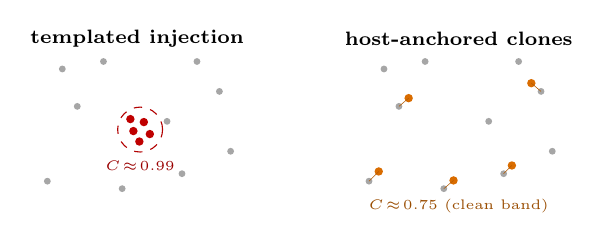
\begin{tikzpicture}[font=\scriptsize, scale=0.95, every node/.style={inner sep=1pt}]
% --- panel A: templated ---
\begin{scope}
\node[font=\scriptsize\bfseries] at (1.35,2.25) {templated injection};
\foreach \x/\y in {0.15/0.35,0.55/1.35,0.35/1.85,1.15/0.25,1.95/0.45,2.45/1.55,2.6/0.75,0.9/1.95,2.15/1.95,1.75/1.15}
  \fill[black!35] (\x,\y) circle (1.3pt);
\foreach \x/\y in {1.30/1.02,1.44/1.14,1.38/0.88,1.52/0.98,1.26/1.18}
  \fill[red!75!black] (\x,\y) circle (1.6pt);
\draw[red!70!black, dashed] (1.39,1.04) circle (0.30);
\node[red!60!black, font=\tiny] at (1.39,0.55) {$C\!\approx\!0.99$};
\end{scope}
% --- panel B: host-anchored clones ---
\begin{scope}[xshift=4.3cm]
\node[font=\scriptsize\bfseries] at (1.35,2.25) {host-anchored clones};
\foreach \x/\y in {0.15/0.35,0.55/1.35,0.35/1.85,1.15/0.25,1.95/0.45,2.45/1.55,2.6/0.75,0.9/1.95,2.15/1.95,1.75/1.15}
  \fill[black!35] (\x,\y) circle (1.3pt);
\foreach \x/\y in {0.28/0.48,0.68/1.46,1.28/0.36,2.06/0.56,2.32/1.66}
  \fill[orange!85!black] (\x,\y) circle (1.6pt);
\foreach \a/\b/\c/\d in {0.15/0.35/0.28/0.48, 0.55/1.35/0.68/1.46, 1.15/0.25/1.28/0.36, 1.95/0.45/2.06/0.56, 2.45/1.55/2.32/1.66}
  \draw[orange!70!black, very thin] (\a,\b) -- (\c,\d);
\node[orange!60!black, font=\tiny] at (1.35,0.02) {$C\!\approx\!0.75$ (clean band)};
\end{scope}
\end{tikzpicture}
\caption{Why the signal works, and where it stops. Grey points are benign documents. \emph{Left:}
passages generated from a shared recipe land on top of each other, so each one's $K$ nearest
neighbours are its own siblings and its neighbourhood coherence is near $1$. \emph{Right:} a
host-anchored clone is placed beside a \emph{different} benign document, so its neighbourhood is
that host's neighbourhood and its coherence is indistinguishable from clean text---the attack is
retrieved just as reliably and the gate never fires (\S\ref{subsec:boundary}).}
\label{fig:geometry}
\end{figure}

\begin{figure}[t]
\centering
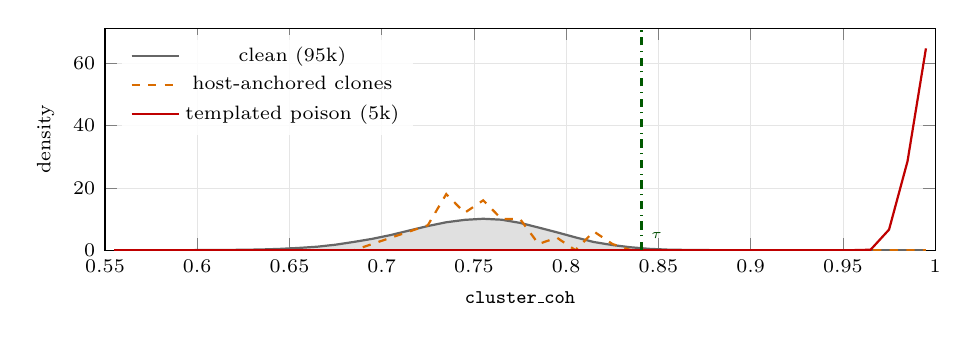
\begin{tikzpicture}
\begin{axis}[
  width=\columnwidth, height=4.4cm,
  xlabel={\texttt{cluster\_coh}}, ylabel={density},
  xmin=0.55, xmax=1.0, ymin=0,
  tick label style={font=\scriptsize}, label style={font=\scriptsize},
  legend style={font=\scriptsize, at={(0.02,0.97)}, anchor=north west, draw=none,
                fill=white, fill opacity=0.85, text opacity=1},
  grid=both, grid style={line width=.2pt, draw=gray!20},
]
\addplot[thick, black!60, fill=black!12, mark=none] coordinates {(0.5550,0.0000) (0.5650,0.0000) (0.5750,0.0011) (0.5850,0.0011) (0.5950,0.0158) (0.6050,0.0253) (0.6150,0.0621) (0.6250,0.1253) (0.6350,0.2232) (0.6450,0.4179) (0.6550,0.7179) (0.6650,1.1084) (0.6750,1.7568) (0.6850,2.6558) (0.6950,3.6505) (0.7050,4.8695) (0.7150,6.3200) (0.7250,7.7400) (0.7350,8.9579) (0.7450,9.7274) (0.7550,10.0789) (0.7650,9.7768) (0.7750,8.7526) (0.7850,7.2663) (0.7950,5.7263) (0.8050,4.1063) (0.8150,2.6137) (0.8250,1.6463) (0.8350,0.9211) (0.8450,0.4263) (0.8550,0.1716) (0.8650,0.0758) (0.8750,0.0211) (0.8850,0.0137) (0.8950,0.0053) (0.9050,0.0011) (0.9150,0.0021) (0.9250,0.0000) (0.9350,0.0000) (0.9450,0.0000) (0.9550,0.0000) (0.9650,0.0000) (0.9750,0.0042) (0.9850,0.0084) (0.9950,0.0063)};
\addlegendentry{clean ($95$k)}
\addplot[thick, orange!85!black, mark=none, dashed] coordinates {(0.5550,0.0000) (0.5650,0.0000) (0.5750,0.0000) (0.5850,0.0000) (0.5950,0.0000) (0.6050,0.0000) (0.6150,0.0000) (0.6250,0.0000) (0.6350,0.0000) (0.6450,0.0000) (0.6550,0.0000) (0.6650,0.0000) (0.6750,0.0000) (0.6850,0.0000) (0.6950,2.0000) (0.7050,4.0000) (0.7150,6.0000) (0.7250,8.0000) (0.7350,18.0000) (0.7450,12.0000) (0.7550,16.0000) (0.7650,10.0000) (0.7750,10.0000) (0.7850,2.0000) (0.7950,4.0000) (0.8050,0.0000) (0.8150,6.0000) (0.8250,2.0000) (0.8350,0.0000) (0.8450,0.0000) (0.8550,0.0000) (0.8650,0.0000) (0.8750,0.0000) (0.8850,0.0000) (0.8950,0.0000) (0.9050,0.0000) (0.9150,0.0000) (0.9250,0.0000) (0.9350,0.0000) (0.9450,0.0000) (0.9550,0.0000) (0.9650,0.0000) (0.9750,0.0000) (0.9850,0.0000) (0.9950,0.0000)};
\addlegendentry{host-anchored clones}
\addplot[thick, red!75!black, mark=none] coordinates {(0.5550,0.0000) (0.5650,0.0000) (0.5750,0.0000) (0.5850,0.0000) (0.5950,0.0000) (0.6050,0.0000) (0.6150,0.0000) (0.6250,0.0000) (0.6350,0.0000) (0.6450,0.0000) (0.6550,0.0000) (0.6650,0.0000) (0.6750,0.0000) (0.6850,0.0000) (0.6950,0.0000) (0.7050,0.0000) (0.7150,0.0000) (0.7250,0.0000) (0.7350,0.0000) (0.7450,0.0000) (0.7550,0.0000) (0.7650,0.0000) (0.7750,0.0000) (0.7850,0.0000) (0.7950,0.0000) (0.8050,0.0000) (0.8150,0.0000) (0.8250,0.0000) (0.8350,0.0000) (0.8450,0.0000) (0.8550,0.0000) (0.8650,0.0000) (0.8750,0.0000) (0.8850,0.0000) (0.8950,0.0000) (0.9050,0.0000) (0.9150,0.0000) (0.9250,0.0000) (0.9350,0.0000) (0.9450,0.0000) (0.9550,0.0000) (0.9650,0.1400) (0.9750,6.6000) (0.9850,28.5000) (0.9950,64.7600)};
\addlegendentry{templated poison ($5$k)}
\draw[green!35!black, dash dot, thick] (axis cs:0.8408,0) -- (axis cs:0.8408,\pgfkeysvalueof{/pgfplots/ymax});
\node[green!30!black, font=\tiny, anchor=south west] at (axis cs:0.8408,0.6) {$\tau$};
\end{axis}
\end{tikzpicture}
\caption{The separation the gate exploits, and the one it misses, on the in-domain corpus.
Templated poison concentrates near $0.99$, entirely above the non-oracle threshold
$\tau=0.841$. Host-anchored clones sit at $0.751$---inside the clean distribution, not merely
near it---which is why no threshold on this statistic can separate them without discarding the
corpus.}
\label{fig:dist}
\end{figure}
SEVA's detection rests on a single per-document statistic. For a document $d$,
let $N_K(d)$ be its $K$ nearest neighbours in the \emph{corpus} embedding space
($K=5$, cosine). The \emph{cluster coherence} of $d$ is the mean pairwise cosine
similarity among those neighbours:
\[
\texttt{cluster\_coh}(d) = \frac{2}{K(K-1)}
\sum_{\substack{d_i,d_j \in N_K(d)\\ i<j}} \cos\!\big(f(d_i),f(d_j)\big).
\]
This is a density-based, $k$-nearest-neighbour cohesion statistic in the lineage of
local-outlier detection~\cite{lof}, but inverted: templated poison is anomalous
precisely because it is \emph{more} locally cohesive than organic text.
Two properties make this robust. First, it is computed over the corpus, not the
per-query retrieval window, and is precomputed and cached as a corpus-level
statistic; it is therefore immune to retrieval-time contamination---an adversary
cannot change a document's coherence through what else is injected for a query.
Second, retrieval over-fetches $K_{\mathrm{FETCH}}=20$ candidates and reranks to
the top $K=5$, so the signal reads a stable neighbourhood. Because $K=5$ is tiny
relative to a $100{,}000$-document corpus, the nearest neighbours of a templated
poison passage are almost exclusively \emph{other passages from the same injected
cluster}, whatever fraction of the corpus is poisoned. In-domain we observe clean
coherence $\approx 0.75$ and templated-poison coherence $\approx 0.99$, a gap of
$+0.235$ to $+0.247$ (SNR $5.8$--$6.0$) that is essentially flat across $1$--$10\%$
contamination (Table~\ref{tab:coh}).
Computing the statistic is a one-time $O(NK)$ pass over the corpus index, amortized
across all subsequent queries; because embeddings are $\ell_2$-normalized, each
cosine is an inner product, and the marginal cost at detection time is a
constant-size threshold test over the documents the RAG system already retrieves.

\subsection{The Hard Gate and Per-Query Aggregation}
SEVA flags a document when its cluster coherence exceeds a calibrated threshold
$\tau$, and flags a \emph{query} as poisoned when at least $k$ of its retrieved
documents are flagged (Algorithm~\ref{alg:seva}). Operating the geometric signal
as a hard gate---rather than as one term in a weighted score---is what gives SEVA
its adaptive robustness (Section~\ref{sec:eval}): an adversary who normalizes soft
linguistic statistics changes nothing about the embedding geometry the gate
reads. Per-query aggregation at $k=2$ exploits the attack's own structure---%
PoisonedRAG injects five passages per target query, so a real attack
lights up several retrieved documents while benign false positives are typically
isolated; requiring two flags cuts the benign query-level false-positive rate
$3.5\times$ at no cost to detection.

\begin{algorithm}[t]
\caption{SEVA detection (\texttt{cluster\_coh} hard gate)}
\label{alg:seva}
\begin{algorithmic}[1]
\REQUIRE corpus $D$; query $q$; threshold $\tau$; aggregation $k$
\REQUIRE precomputed $C[d]=\texttt{cluster\_coh}(d)$ for all $d\in D$
\STATE $R \leftarrow$ rerank top-$K$ of $\mathrm{Retrieve}_{K_{\mathrm{FETCH}}}(q, D)$
\STATE $\mathit{flags} \leftarrow \big|\{\, d \in R : C[d] > \tau \,\}\big|$
\IF{$\mathit{flags} \ge k$}
\RETURN \textsc{Flag} \quad (query poisoned)
\ELSE
\RETURN \textsc{Pass}
\ENDIF
\end{algorithmic}
\end{algorithm}

\subsection{Density-Agnostic, Non-Oracle Calibration}
SEVA's threshold is calibrated with no knowledge of the poison, in two phases over
a fixed pool of benign queries. In the \emph{calibration} phase, benign queries are
issued against the (possibly poisoned) corpus; for every retrieved document the
detection score is computed, and $\tau$ is set to the
$(1-\mathrm{FPR}_{\mathrm{TARGET}})$ quantile of the resulting clean-score
distribution by 50-iteration binary search, with
$\mathrm{FPR}_{\mathrm{TARGET}}=0.69\%$. In-domain this places the geometric gate at
$\tau\approx0.84$---far below templated poison's $\approx\!0.99$ coherence and well
above clean documents' $\approx\!0.75$. In the \emph{evaluation} phase, the
remaining benign queries and all adversarial queries are scored against the frozen
$\tau$; documents seen during calibration are excluded from false-positive
accounting (decontamination), so a document cannot improve the measured rate by
having been calibrated on.

Two assumptions are explicit. First, calibration uses \emph{no labeled poison and
no oracle knowledge of the contamination density}: $\tau$ is a function of the
clean-score quantile alone. This is what makes the protocol deployable---an operator
sets a target false-positive rate, not a guess at how poisoned the corpus is.
Second, calibration assumes the benign query stream is itself uncontaminated, which
holds under the threat model of Section~\ref{sec:threat}: the adversary has
corpus-write access, not control of the operator's own calibration queries. SEVA
exploits exactly this asymmetry between a contaminable corpus and a clean query
channel.

We validate the protocol under its hardest version. Rather than calibrate on the
same poison we evaluate, we fit the threshold (and, for the composite ablation, the
signal weights) on a \emph{disjoint reference half} of the templated attack,
\emph{freeze} it, and deploy unchanged on a held-out half. The frozen detector
catches the held-out poison at $0\%$ poison-evasion and $0.58\%$ document-FPR
(Section~\ref{subsec:main}), establishing that detection is not an oracle artifact
of tuning on the test poison.

\subsection{The Multi-Signal Composite as Ablation}
SEVA began as a ten-signal detector that combined cluster coherence with soft
linguistic and structural statistics through SNR-weighted, log-capped fusion:
weights $w_i \propto \min\!\big(\log(1+|\mathrm{SNR}_i|),\,c\big)$ over the nine
signals that clear an $|\mathrm{SNR}|\geq0.5$ gate, with automatic polarity
inversion for signals (such as type--token ratio) that run lower on poison.
The supplementary material gives the full signal inventory and its in-domain separation. The
design held up against a general-domain corpus and a naive adversary; the
evaluation gauntlet---an in-domain corpus that removes the domain shortcut, plus an
adaptive adversary---is what exposed it.

Two failures, both visible in that inventory. First, the soft signals are
\emph{domain-confounded}: keyword density, the strongest of them, separates poison
from clean at an SNR of $38$ against a general-domain background but only
$\approx\!8$ in-domain, because much of its apparent power was discriminating
security text from Wikipedia, not poison from clean.
Second, they are \emph{normalizable}: a keyword-dropping adversary neutralizes them
at the feature level, driving the composite's poison-evasion to $49$--$57\%$
(Section~\ref{subsec:core}), because cluster coherence carries too little of the
fused weight ($\approx\!0.15$) to hold the score alone.
Only cluster coherence is both domain-robust---its SNR \emph{rises} in-domain---and
adaptation-robust, reading geometry an adversary cannot normalize without
sacrificing the retrievability the attack needs. We therefore distilled SEVA to
this single signal and report the composite as the ablation that quantifies what
the soft signals cost. The deployed detector is the hard cluster-coherence gate: no
LLM, CPU-only, one precomputed statistic.

\section{Evaluation}
\label{sec:eval}
\subsection{Experimental Setup}

\noindent\textbf{Corpora.} We evaluate on three corpora chosen to stress
different failure modes. The primary corpus is an in-domain Security Stack
Exchange question--answer corpus of $100{,}000$ documents, deduplicated, with
whole-corpus clean cluster-coherence $0.705$ (the mean over retrieved evaluation
neighbourhoods, the quantity Table~\ref{tab:coh} reports, is $\approx\!0.75$).
It is a deliberate \emph{domain-confound control}: clean and poison are drawn from
the same security domain, so a detector relying on topic contrast---security text
against general-domain prose---is denied its shortcut. Most prior defense
evaluations inject security- or instruction-style poison into a general-domain
background, which inflates linguistic-signal separation; we remove that confound.
The two cross-domain corpora are Natural Questions~\cite{nq} and
HotpotQA~\cite{hotpotqa}, each an $\approx\!150{,}000$-passage subsample of the
BEIR corpus~\cite{beir} (a per-query Contriever~\cite{contriever} neighbourhood plus
a random background). They differ sharply in benign duplication---$1.15\%$ and $9.06\%$ of
clean documents share a 5-gram with another, against $0.24\%$ in the Security
corpus---the property that separates lexical from semantic detection
(\S\ref{subsec:lex}).

\noindent\textbf{Attacks.} On the in-domain corpus we inject \emph{templated}
poison---multiple passages per target query from a shared security-domain recipe,
at $1\%$, $5\%$, and $10\%$ contamination---and model the adaptive adversary by
ablating the soft signals an attacker can normalize: keyword density (tier L2) and
keyword density plus sentence structure (tier L3). Because PoisonedRAG releases
poison only for general-domain benchmarks, the in-domain corpus additionally
receives a faithful black-box PoisonedRAG generated with the authors' released
attack code (used in the cross-corpus comparison, \S\ref{subsec:lex}). On the
cross-domain corpora we inject the \emph{released} PoisonedRAG attack: the attack
authors' own published
adversarial passages~\cite{poisonedrag} ($100$ target queries $\times\,5$
passages), built to their released construction (the target question prepended to
an LLM-crafted payload). Released poison removes any question of a favourable
re-implementation.

\noindent\textbf{Detector, metrics, protocol.} All documents are embedded with
BAAI/bge-large-en-v1.5 ($1024$-d, normalized)~\cite{bge} and indexed with FAISS
HNSW~\cite{faiss,hnsw} ($M=32$, $\mathrm{efConstruction}=200$). We report the
poison-evasion rate $\mathrm{FN}/(\mathrm{TP}+\mathrm{FN})$---the fraction of
templated poison the gate fails to flag, i.e.\ one minus the catch rate---and the
document false-positive rate $\mathrm{FPR}=\mathrm{FP}/(\mathrm{FP}+\mathrm{TN})$
against a universal target $\mathrm{FPR}_{\mathrm{TARGET}}=0.69\%$. Thresholds are
calibrated on benign queries only---no labeled poison, no oracle density---and
documents seen during calibration are excluded from false-positive counting.
In-domain results use three calibration-partition seeds ($42$, $7$, $123$) over a
fixed pool of $2{,}000$ benign queries; cross-domain results use the released
poison at seed $42$. Numbers are measured on an RTX 5080 (CUDA); detection and
latency are additionally reproduced on an RTX 4060 and an Apple M4
(\S\ref{subsec:eff}).

\subsection{Primary Detection Results}
\label{subsec:main}

\begin{figure}[t]
\centering
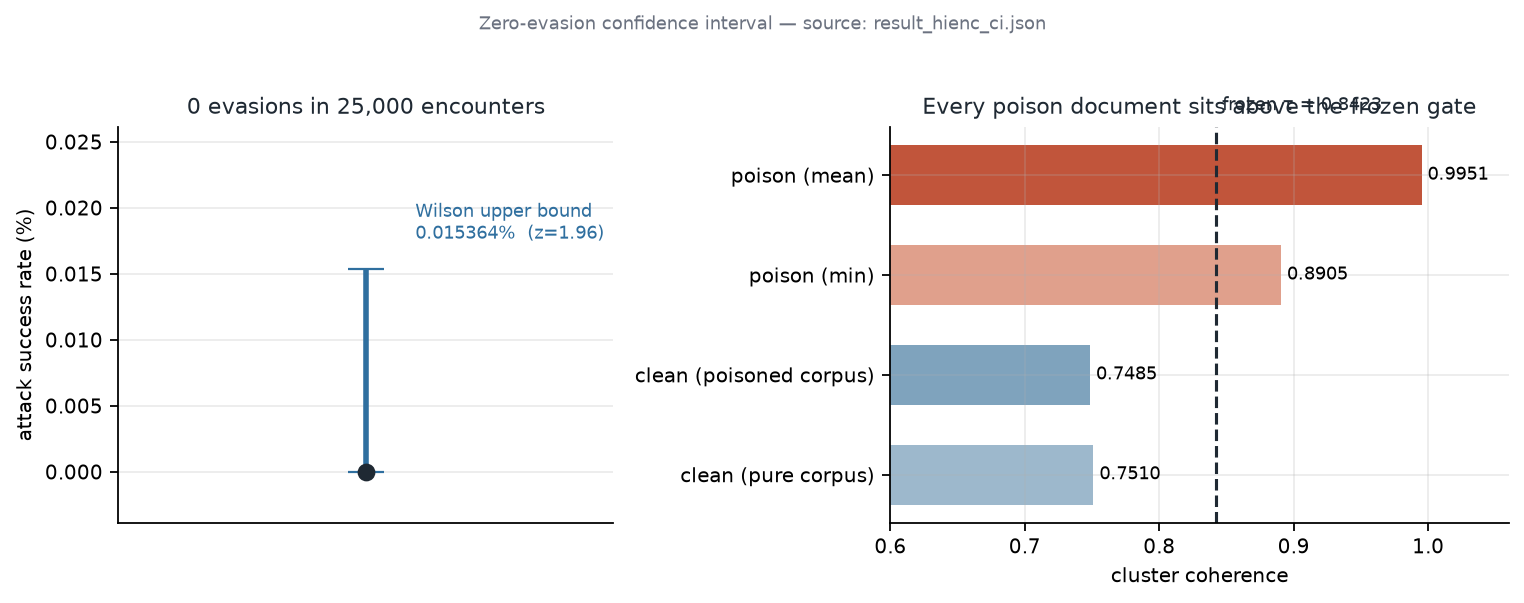
\includegraphics[width=\columnwidth]{docs/figures/confidence_interval.png}
\caption{Zero evasion with its confidence bound. \emph{Left:} $0$ evasions in $25{,}000$ high-encounter trials gives a $95\%$ Wilson upper bound of $0.0154\%$. \emph{Right:} every poison document sits above the frozen $\tau=0.8423$---minimum poison coherence $0.8905$ against a clean mean of $0.7510$---which is why the interval is that tight.}
\label{fig:ci}
\end{figure}
Table~\ref{tab:main} is the central result: SEVA across three adversary tiers,
three contamination densities, and three calibration seeds on the in-domain
corpus. At L1---the full signal set against a naive templated adversary---SEVA
flags every injected passage: \textbf{$0\%$ poison-evasion across all nine
conditions}, with a dedicated high-encounter run tightening the $95\%$ Wilson upper
bound to $0.0154\%$ ($0$ evasions in $25{,}000$ templated encounters at the frozen
gate), at a document false-positive rate held near the $0.69\%$ target (grand mean
$0.56\%$ across the nine conditions; the frozen disjoint-reference protocol of
\S\ref{subsec:geom} reports a comparable $0.58\%$; per-condition maximum $0.83\%$ on the
high-variance seed~7).
Two things make this result load-bearing rather than incidental. First, because
clean and poison are drawn from the \emph{same} security domain, $0\%$ cannot be a
domain-contrast artifact---the very confound that flatters linguistic detectors
when poison is security text on a general-domain background (\S\ref{subsec:geom}).
Second, it is not a single lucky split: the $0\%$ is identical at all three seeds
and every density. The complete per-condition breakdown---all nine
density$\times$seed cells, with document- and query-level false-positive rates and
$95\%$ Wilson upper bounds on the $0\%$ poison-evasion---is given in the
supplementary material (per-seed confusion matrices and per-condition rates).

Tiers L2 and L3 ablate the soft keyword and sentence-structure signals to model
the keyword-dropping adaptive adversary (\S\ref{sec:threat}). Here the multi-signal
composite's poison-evasion rises to $42$--$72\%$, climbing with density
(Table~\ref{tab:main})---the cost of \emph{ablating} those signals from the detector,
complementary to the feature-neutralization attack against the full composite quantified
in \S\ref{subsec:core}.
This is the central negative finding of our own evaluation, and we put it in the
primary table rather than a footnote: \emph{the soft signals do not survive
adaptation}. The apparent multi-signal robustness of a permissive evaluation is,
in-domain, carried almost entirely by a single normalizable signal. We make this
the hinge of the architecture (\S\ref{subsec:core}): the geometric core, operated
as a hard gate, holds $0\%$ on exactly these adaptive conditions. The
false-positive rate, by contrast, stays near target across every tier and density
(all rows $0.52$--$0.63\%$ mean), because $\tau$ is recalibrated per condition to
the clean-score quantile---the L2/L3 detection collapse is not bought back by
spending false positives.

\begin{table}[t]
\centering
\caption{Primary in-domain results: Security Stack Exchange, $100{,}000$
documents, mean\,$\pm$\,sample std ($n=3$ seeds). L1 is the full signal set (naive
adversary); L2/L3 ablate the soft signals to model the keyword-dropping adaptive
adversary. SEVA catches \emph{all} templated poison at L1 ($0\%$ poison-evasion)
across every density and seed; the L2/L3 rise is the composite's adaptive collapse---the
ablation of \S\ref{subsec:core}, which the geometric hard gate eliminates
($0\%$, \S\ref{subsec:core}).}
\label{tab:main}
\begin{tabular}{llcc}
\toprule
Tier & Density & Evasion (\%) & Doc-FPR (\%) \\
\midrule
\multirow{3}{*}{L1 (naive)}    & 1\%  & $\mathbf{0.0\pm0.0}$ & $0.54\pm0.17$ \\
                               & 5\%  & $\mathbf{0.0\pm0.0}$ & $0.63\pm0.18$ \\
                               & 10\% & $\mathbf{0.0\pm0.0}$ & $0.52\pm0.15$ \\
\midrule
\multirow{3}{*}{L2 (adaptive)} & 1\%  & $44.0\pm1.4$ & $0.53\pm0.21$ \\
                               & 5\%  & $57.0\pm6.7$ & $0.59\pm0.21$ \\
                               & 10\% & $72.4\pm1.1$ & $0.52\pm0.22$ \\
\midrule
\multirow{3}{*}{L3 (adaptive)} & 1\%  & $42.4\pm2.8$ & $0.58\pm0.18$ \\
                               & 5\%  & $57.0\pm6.7$ & $0.59\pm0.21$ \\
                               & 10\% & $72.4\pm1.1$ & $0.52\pm0.22$ \\
\bottomrule
\end{tabular}
\end{table}

\subsection{Density-Invariant Geometry}
\label{subsec:geom}
The signal underlying the L1 result is the cluster-coherence gap
(Table~\ref{tab:coh}): in-domain, clean documents sit at coherence $\approx 0.75$
and templated poison at $\approx 0.99$, and the separation does not move with
contamination density. We state this as a formal property of the attack geometry.

\smallskip
\noindent\textbf{Observation~1 (Geometric Invariance of Cluster Coherence).}
\emph{For templated, multi-passage corpus injection in a $100{,}000$-document
corpus scored with $K=5$ nearest neighbours, the per-document cluster-coherence gap
(poison mean $-$ clean mean) is invariant to contamination density across the
evaluated $1$--$10\%$ range.}

\emph{Evidence.} The gap is $+0.235$, $+0.238$, and $+0.247$ at $1\%$, $5\%$, and
$10\%$ density---a total spread of $0.012$---at an SNR of $5.99$, $6.00$, and $5.78$
(Table~\ref{tab:coh}); neither quantity shows systematic density dependence. It is
equally seed-invariant: the gap is identical across calibration seeds $42$, $7$, and
$123$, because it is a property of the corpus and the injected cluster, not of the
benign calibration split.

\emph{Mechanism.} Cluster coherence measures a local geometric property of the
injection itself---the tightness of the embedding region the templated passages
occupy. Because $K=5$ is tiny relative to $100{,}000$ documents, a poison document's
$K$ nearest neighbours are almost exclusively its own injected siblings, whatever
fraction of the corpus is poisoned; the gap therefore reflects between-sibling
template homogeneity, not relative population statistics. This is exactly what a
pairwise deduplicator cannot see: comparing two documents at a time, it has no
notion of the cluster a multi-passage injection forms, and no reason for its
separation to stay stable as that cluster grows.

\emph{Intrinsic, not domain-induced.} The in-domain SNR ($5.8$--$6.0$) \emph{exceeds}
the $\approx\!4.7$ the same signal records against a general-domain corpus
(WikiText-103~\cite{wikitext}). Cluster coherence is therefore not a domain-contrast
artifact: in-domain, where the soft linguistic signals lose most of their apparent
power, the geometric gap is if anything \emph{wider}. The
very domain confound that inflates the linguistic signals is, for the geometric one,
evidence that the separation is a property of the templating process rather than of
the topic.

\emph{Scope.} The invariance is established over the evaluated $1$--$10\%$ range,
which we neither evaluate beyond nor extrapolate.

Frozen, non-oracle, held-out calibration confirms the operational consequence: a
threshold fit on a disjoint reference half of the attack and then frozen catches the
held-out half at $0\%$ poison-evasion and $0.58\%$ document-FPR.

\begin{table}[t]
\centering
\caption{In-domain \texttt{cluster\_coh} geometry across contamination density
(Security Stack Exchange, $100{,}000$ documents). The poison--clean gap and its
SNR are density-invariant and \emph{larger} than the $\approx\!4.7$ SNR the same
signal shows against a general-domain corpus---the gap reads template homogeneity,
not domain contrast. The encoder-invariance and cross-platform results
(\S\ref{subsec:encoder}, \S\ref{subsec:eff}) report an independently re-embedded measurement of
this bge geometry, agreeing with the values here up to third-decimal re-embedding differences.}
\label{tab:coh}
\begin{tabular}{lcccc}
\toprule
Density & Clean coh. & Poison coh. & Gap & SNR \\
\midrule
1\%  & 0.7518 & 0.9871 & $+0.2353$ & 5.99 \\
5\%  & 0.7526 & 0.9909 & $+0.2384$ & 6.00 \\
10\% & 0.7466 & 0.9939 & $+0.2474$ & 5.78 \\
\bottomrule
\end{tabular}
\end{table}

\subsection{Calibration Scaling}
\label{subsec:calib}

\begin{figure}[t]
\centering
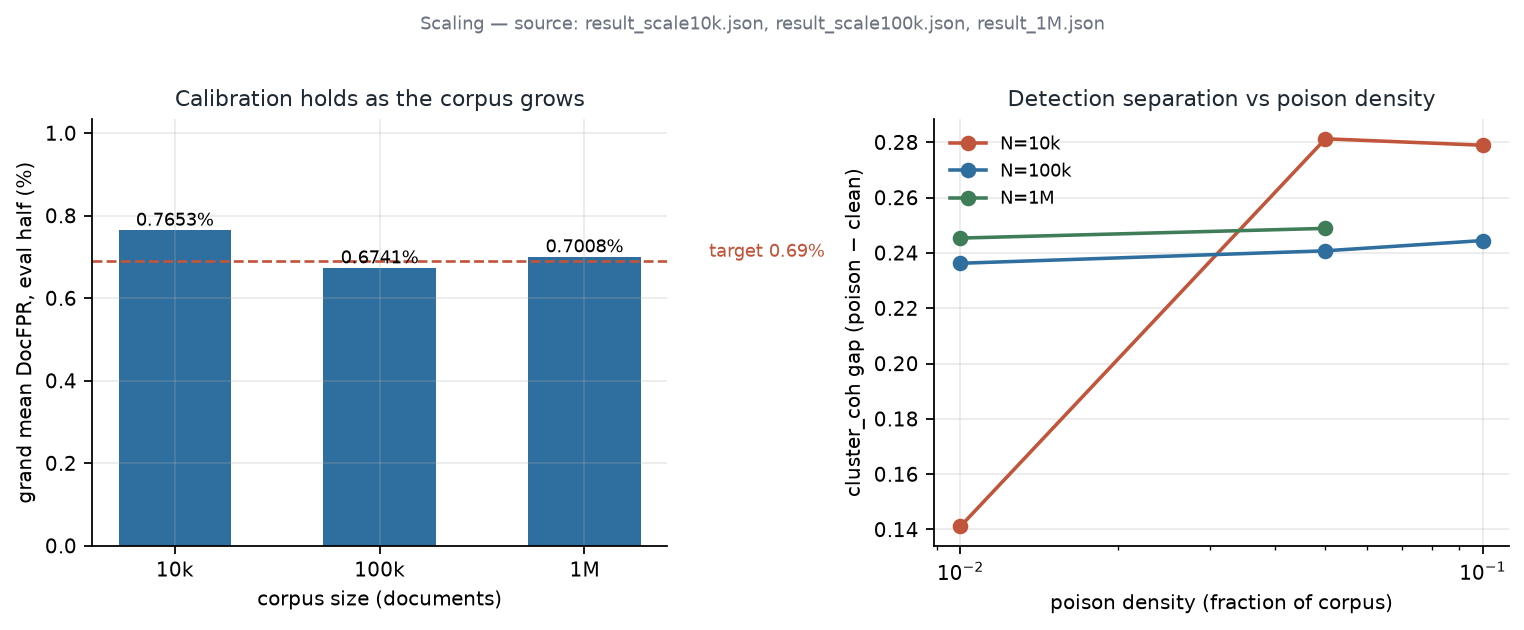
\includegraphics[width=\columnwidth]{docs/figures/scaling.png}
\caption{Calibration scaling and density-invariance across corpus size. \emph{Left:} realized non-oracle document-FPR against the $0.69\%$ target at $10$k, $100$k and $1$M---the deviation does not grow with $N$ (Observation~2). \emph{Right:} the cluster-coherence gap per contamination density; the $100$k and $1$M curves are flat, while at $10$k the gap collapses at $1\%$ density. Density-invariance is a large-corpus property, and we plot where it fails rather than omitting it.}
\label{fig:scaling}
\end{figure}
The deployed threshold $\tau$ is calibrated non-oracle, as the $(1-0.0069)$
empirical percentile of clean coherence. A second formal property governs how
tightly its realized false-positive rate tracks that $0.69\%$ target as the clean
calibration corpus grows.

\smallskip
\noindent\textbf{Observation~2 (Calibration Scaling).}
\emph{The realized non-oracle document false-positive rate converges toward the
calibration target ($0.69\%$) as the clean calibration corpus grows; its deviation
from the target shrinks with corpus size.}

\emph{Evidence.} The grand-mean held-out document-FPR is $0.765\%$ at $N=10{,}000$,
$0.674\%$ at $N=100{,}000$, and $0.701\%$ at $N=1{,}000{,}000$---the deviation from the
$0.69\%$ target falling from $0.075\%$ to $0.016\%$ to $0.011\%$ as $N$ grows, at the
frozen $\tau$ (three seeds at each size; the $1$M point uses the broader corpus of
\S\ref{subsec:scale}).

\emph{Mechanism.} $\tau$ is an order statistic of the clean-coherence sample, so the gap
between realized and target FPR is a uniform-convergence quantity. Writing $F$ for the clean
coherence CDF and $F_n$ for its empirical counterpart over $n$ calibration documents, the
realized false-positive rate at the plug-in threshold
$\tau=F_n^{-1}(1-\alpha)$ satisfies
$|\,\mathrm{FPR}(\tau)-\alpha\,| \le \sup_x |F_n(x)-F(x)|$, and by the
Dvoretzky--Kiefer--Wolfowitz inequality~\cite{dkw} this is at most
$\sqrt{\ln(2/\delta)/2n}$ with probability $1-\delta$. The deviation therefore decays as
$O(1/\sqrt{n})$ in the number of \emph{clean} calibration documents---a property of the
calibration set alone, independent of the attack. The bound is distribution-free and hence
loose; we report it for the rate it predicts, which is the trend the three measured points
follow, not as a tight numerical guarantee.

\emph{Scope.} The deviation shrinks at three corpus sizes ($10{,}000$, $100{,}000$,
$1{,}000{,}000$)---the direction the $O(1/\sqrt{N})$ argument implies. Because the
largest point uses a broader corpus (\S\ref{subsec:scale}), we report the direction,
not a fitted exponent, and do not extrapolate the rate.

\subsection{Encoder-Invariance}
\label{subsec:encoder}

\begin{figure}[t]
\centering
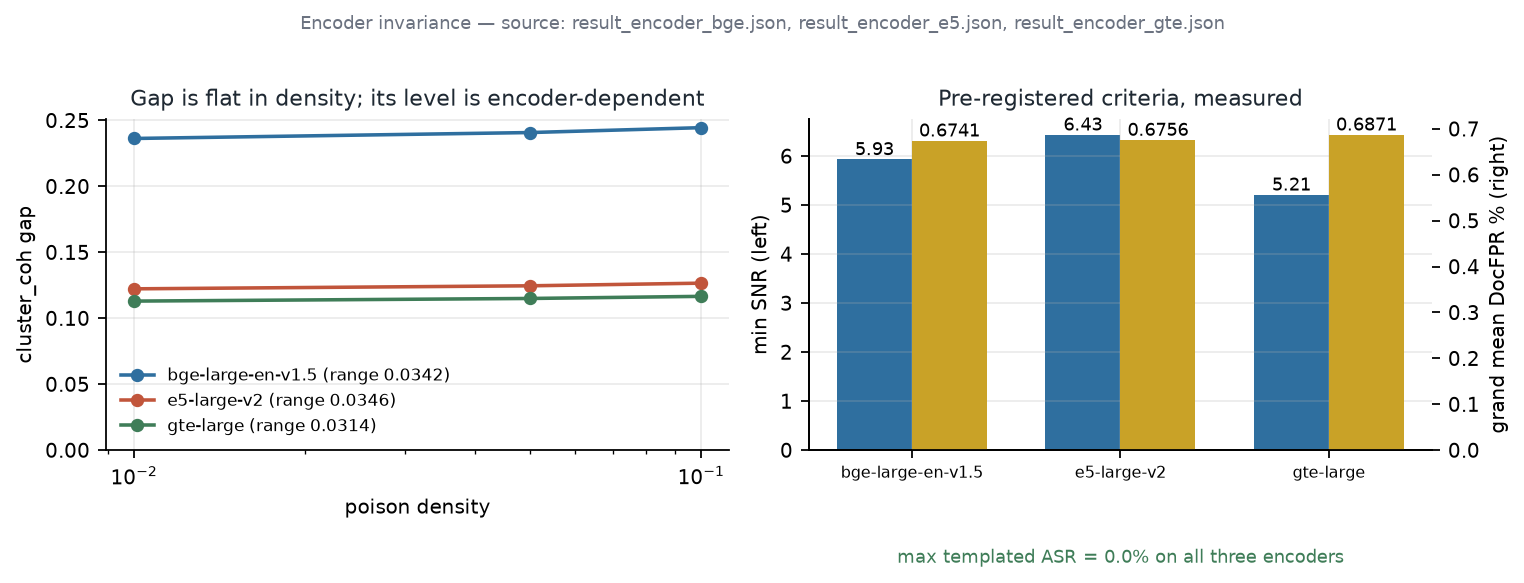
\includegraphics[width=\columnwidth]{docs/figures/encoder_invariance.png}
\caption{Encoder-invariance across three independent pre-training lineages. Each encoder is flat in density (relative gap range $\le 0.035$) and reaches $0\%$ templated poison-evasion, but the \emph{absolute} separation is encoder-dependent (bge $\approx 0.24$; e5 $\approx 0.12$; gte $\approx 0.11$). What generalizes is that the gate works, not that the margin is the same size on every manifold.}
\label{fig:encoder}
\end{figure}
The cluster-coherence signal reads similarities in one embedding model's space, so a
fair worry is that it detects that model's idiosyncrasies rather than the attack. It
does not.

\smallskip
\noindent\textbf{Observation~3 (Encoder-Invariance).}
\emph{Templated-poison detection by the geometric gate is a property of the attack,
not of one encoder: across embedding models of independent pre-training lineages, each
used in its correct symmetric convention and calibrated non-oracle on its own clean
coherence, the gate catches all templated poison ($0\%$ poison-evasion), density-invariantly, at
preserved signal-to-noise.}

\emph{Evidence.} Re-embedding the identical hash-verified corpus with three encoders of
distinct lineages---bge-large~\cite{bge} (BAAI), e5-large-v2~\cite{e5} (Microsoft), and
gte-large~\cite{gte} (Alibaba)---and re-deriving the non-oracle threshold on each
encoder's clean coherence, templated poison sits at cohesion $\approx 0.99$ under all
three; poison-evasion is $0\%$ on all nine conditions for every encoder, the gap is
density-invariant (range $\le 3.5\%$ of its mean), and the document-FPR holds near the
$0.69\%$ target.

\emph{Mechanism.} Templated passages are near-duplicates, and near-duplicate texts map
to near-identical vectors under any competent encoder; they form a tight local
cluster---high cohesion---whatever manifold the encoder induces. The \emph{absolute}
gap does shrink across the three ($+0.236 \to +0.123 \to +0.115$), but only because
their clean manifolds are progressively more concentrated (clean coherence
$0.751 \to 0.866 \to 0.881$); the poison cohesion stays pinned at $\approx 0.99$ and
the scale-normalized separation (SNR $5.2$--$6.7$) is preserved. The gate keys on the
geometry of the injection, not the idiosyncrasy of one representation.

\emph{Scope.} Established on three encoders of independent lineages, each used in its
correct \emph{symmetric} convention (bge and gte take no instruction prefix; e5 takes
its symmetric ``query:''\ prefix on all texts); because absolute cohesion scales with
the manifold, SNR is the cross-encoder comparator. We do not claim invariance to
deliberately poison-aware or adversarially-trained embeddings.

\subsection{Cross-Domain Detection on Released PoisonedRAG}
The in-domain result establishes that SEVA catches templated poison; the
cross-domain results establish that it catches the \emph{published} attack on
benchmarks it never calibrated against. On PoisonedRAG's released adversarial
passages for Natural Questions and HotpotQA---and a faithful black-box PoisonedRAG,
built with the authors' \emph{released} attack code, on the in-domain Security
corpus---SEVA flags
the attack at the $0.69\%$ non-oracle operating point, catching $98\%$ (Security),
$82\%$ (Natural Questions), and $97\%$ (HotpotQA) of the injected poison---a poison-evasion rate of $2\%$, $18\%$, and $3\%$
respectively. These are \emph{detection} rates, the fraction of poison the gate
flags, not end-to-end answer-corruption: PoisonedRAG's released passages are
engineered for high end-to-end attack-success against a generator in the
loop~\cite{poisonedrag}, and SEVA---run purely as a detector---removes the great
majority of them from the retrieval set before any generator is invoked. The two are
distinct quantities, and we do not plot one against the other.
The threshold is fit on each corpus's clean documents alone, with no sight of the
poison, so this is detection under deployment conditions, not oracle tuning. And
because the cross-domain passages are the attack authors' \emph{released} artifacts
on the field's own benchmarks, the result forecloses the obvious objection that a
defense works only
against its designers' own re-implementation of the attack: SEVA detects
PoisonedRAG on the ground PoisonedRAG was built to win.

\subsection{Lexical Duplicate Filtering Is Corpus-Fragile}
\label{subsec:lex} also answers the sharpest objection to a cohesion-based detector: that
it merely reimplements the duplicate filtering PoisonedRAG itself tested and dismissed
(\S7.3 of~\cite{poisonedrag}). Lexical near-duplicate filtering (MinHash~\cite{minhash}) is \emph{corpus-fragile}. On the lexically
sparse Security corpus it catches the attack ($98\%$), because a matched-FPR threshold can sit
low enough to flag the injected passages' shared $n$-grams. But on Natural Questions and
HotpotQA---whose benign duplication is $5\times$ and $38\times$ higher---holding the same
$0.69\%$ false-positive rate forces the threshold \emph{above} the injected overlap and the
filter catches \emph{nothing} ($0\%$ at every deployable FPR below $2\%$), while cluster
coherence still catches $82$--$97\%$. Its effectiveness is thus a property of the corpus, not of
the attack---the fragility \S7.3 of PoisonedRAG observed without diagnosing.

Embedding near-duplicate detection ($s_{nd}$, maximum cosine to the nearest corpus neighbour) is
the stronger baseline and we hold ourselves to it honestly: it is competitive ($52/98/98\%$
across the three corpora), and cluster coherence's advantage is corpus-dependent---a clear
margin on Natural Questions ($82\%$ vs.\ $52\%$), parity elsewhere. The reason traces to
\S\ref{subsec:geom}: $s_{nd}$ asks whether a passage has one near-twin, cluster coherence
whether it sits inside a tight \emph{group}. The two coincide when the injected cluster is dense
and dominant, and diverge when its members are individually unlike any single clean document but
collectively cohesive. Our claim is scoped accordingly: cluster coherence beats \emph{lexical}
filtering across corpora and matches or exceeds embedding deduplication, with an edge where
benign duplication is moderate.

\subsection{Head-to-Head Against the Per-Query State of the Art}
\label{subsec:h2h}
The deployability claim demands a real comparison, not lifted numbers. We reproduce
RAGDefender---the LLM-free, per-query state of the art~\cite{ragdefender}---on our shared
Security corpus and templated attack, using SEVA's own encoder (bge-large) so the comparison
isolates the \emph{algorithmic} difference. Two findings follow. First,
RAGDefender's clustering filter has no no-attack gate: its grouping step always partitions a
retrieval window and removes a side, so on benign in-domain queries it strips $50.4\%$ of clean
documents---not a deployable operating point, and one invisible to evaluations that never
measure benign-query false positives. Second, to compare \emph{detection} at all we grant it an
idealized threshold its actual filter does not expose, at a matched $\sim$0.8\% benign
false-positive point looser than SEVA's own $\sim$0.6\%---both concessions in its favour. Even
then SEVA catches $100\%$ of templated poison to RAGDefender's $\sim$89\%, which reaches parity
only by spending false positives it cannot afford ($\sim$93\% at $5\%$ FPR, $\sim$98\% at
$50\%$ FPR).
The structural reason is the one that also powers the cross-domain result: cluster
coherence is corpus-level, so it flags a templated passage even when that passage
is the only injected document in a given retrieval window---precisely the case a
per-query view, which can only compare documents co-retrieved for one query, cannot
see.

\subsection{The Geometric Core vs.\ the Composite}
\label{subsec:core}
We now isolate why SEVA deploys the hard gate rather than the
composite that Table~\ref{tab:main} ablates: three attacks, one operating point
($0.69\%$ document-FPR), two detectors. On the naive templated attack both reach
$0\%$ poison-evasion---the composite's soft signals add nothing the geometry does not
already supply. On \emph{real} PoisonedRAG the gap opens: the hard gate catches $98\%$
($2\%$ evasion) while the full SNR-weighted composite catches only $72\%$ ($28\%$ evasion).
The soft signals do not merely fail to help; they \emph{dilute}, pulling the fused
score of genuine poison below threshold.
Under the keyword-dropping adversary---which neutralizes the soft features in the attack
text itself---the dilution becomes collapse: at the frozen operating point the composite's
poison-evasion is $49$--$57\%$, a measurement distinct from the
density-swept $42$--$72\%$ of the ablation tiers (Table~\ref{tab:main}) though it exposes the
same fragility, because cluster coherence carries too little fused weight
($\approx\!0.15$ of the total) to hold the score once keyword density is normalized,
whereas the hard gate---reading only the embedding geometry the adversary never
touches---holds $0\%$: the highest-SNR signals of a permissive evaluation are the
first to fall to an adaptive adversary, and the geometric core is what remains.

A single hard gate raises one deployment concern: document-level false positives,
accumulated over a multi-document retrieval window, inflate the rate at which whole
\emph{queries} are flagged. Per-query aggregation removes it (supplementary material).
Because PoisonedRAG injects five passages per target query, a genuine
attack lights up several retrieved documents while benign false positives are
typically isolated; flagging a query only when $\geq\!2$ of its retrieved documents
gate cuts the benign query-level false-positive rate from $3.15\%$ to
$0.90\%$---a $3.5\times$ reduction---while the poison catch rate is unchanged at
$98\%$.

\begin{figure}[t]
\centering
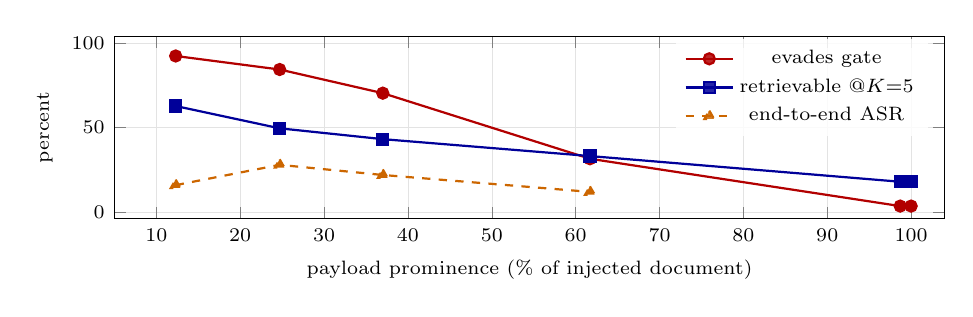
\begin{tikzpicture}
\begin{axis}[
  width=\columnwidth, height=3.9cm,
  xlabel={payload prominence (\% of injected document)},
  ylabel={percent}, ymin=-4, ymax=104, xmin=5, xmax=104,
  ylabel near ticks, xlabel near ticks,
  tick label style={font=\scriptsize}, label style={font=\scriptsize},
  legend style={font=\scriptsize, at={(0.98,0.72)}, anchor=east, draw=none, fill=white, fill opacity=0.85, text opacity=1},
  grid=both, grid style={line width=.2pt, draw=gray!22},
]
\addplot[mark=*, thick, color=red!70!black] coordinates
  {(12.3,92.4) (24.7,84.4) (37.0,70.4) (61.7,31.6) (98.7,3.6) (100,3.6)};
\addlegendentry{evades gate}
\addplot[mark=square*, thick, color=blue!60!black] coordinates
  {(12.3,62.8) (24.7,49.6) (37.0,43.2) (61.7,33.2) (98.7,18.0) (100,18.0)};
\addlegendentry{retrievable @$K{=}5$}
\addplot[mark=triangle*, thick, dashed, color=orange!80!black] coordinates
  {(12.3,16.0) (24.7,28.0) (37.0,22.0) (61.7,12.0)};
\addlegendentry{end-to-end ASR}
\end{axis}
\end{tikzpicture}
\caption{The attacker's frontier over payload prominence (in-domain, seed~42). Raising payload
prominence trades evasion ($92\%\!\to\!4\%$) and retrievability ($63\%\!\to\!18\%$) against
potency, giving an interior optimum at $25\%$ payload where end-to-end success peaks at $28\%$
\emph{and evasion is still total}. The gate only begins to fire beyond that point, so it does
not bind at the operating point an adversary would choose (\S\ref{subsec:boundary}).}
\label{fig:frontier}
\end{figure}

\subsection{The Boundary: Host-Anchored Cloning}
\label{subsec:boundary}
Every result so far concerns injections built from a shared recipe, which is exactly what the
gate reads---so the honest question is what happens when an adversary abandons it. In a
\emph{host-anchored clone}, the attacker rewrites the target's top-ranked benign document with an
offline LLM to preserve meaning while changing surface form, then splices in the payload. Each
injected passage is anchored to a \emph{different} benign document, so its $K$-nearest
neighbours are that host's neighbourhood rather than its own siblings.

The gate does not see this attack. Clone cohesion averages $0.751$ against $\tau=0.841$---below
the gate for \emph{every} one of $50$ targets ($100\%$ poison-evasion), while $84\%$ remain
retrieved at $K=5$. Multiplicity does not rescue detection: $1$ to $5$ clones per target moves
mean cohesion only from $0.722$ to $0.790$, because each embedding is dominated by its distinct
host rather than the shared payload. Nor does the complementary signal: nearest-neighbour
duplication $s_{nd}$, which flags templated poison perfectly, catches only $13$--$20\%$ of
clones, and a two-signal union gate at the same $0.69\%$ budget reaches just $6.7$--$33.3\%$.

\emph{The bypass is not expensive.} It would be convenient to report that evasion costs the
adversary its effect, and we initially expected it to. Measured consistently it does not. Among
the $42$ clones that evade the deployed gate and are retrieved, $31.0\%$ ($13/42$; $95\%$ Wilson
$19.1$--$46.0\%$) corrupt the answer, an end-to-end success rate of $26\%$ over all $50$
targets. On the \emph{same} targets, generator, and corruption criterion, the templated attack
the gate does stop reaches only $18\%$ undefended (\S\ref{subsec:e2e}). Sweeping payload
prominence (Fig.~\ref{fig:frontier}) gives the adversary an interior optimum at $25\%$ payload,
where evasion is still total and end-to-end success peaks at $28\%$; beyond that the gate begins
to fire, but retrievability is already falling, so the optimum is unaffected by whether the gate
is deployed at all. We therefore make no cost-of-attack claim: against an adversary willing to
change strategy, the gate removes the attack it detects without raising the attacker's price.

\emph{The blind spot is shared, not ours.} Reproducing CleanBase~\cite{cleanbase}---the closest
peer, which detects the cliques that co-targeted documents form in a corpus-level similarity
graph---and matching it to the same $0.69\%$ clean false-positive point, it catches $100\%$ of
templated poison and $0\%$ of host-anchored clones: identical to SEVA on both regimes
(Table~\ref{tab:boundary}). Since the two detectors share only the mutual-similarity assumption
and not the statistic computed from it, the boundary is a property of the assumption, and so of
the cohesion-detection family.

\begin{table}[t]
\centering
\caption{Both corpus-level cohesion detectors, at a matched $0.69\%$ clean false-positive point,
on the two injection regimes. They agree exactly: the assumption they share is what fails.}
\label{tab:boundary}
\begin{tabular}{lcc}
\toprule
Detector & Templated & Host-anchored clones \\
\midrule
SEVA (\texttt{cluster\_coh} gate) & \textbf{100\%} & $0\%$ \\
CleanBase~\cite{cleanbase} (reproduced) & \textbf{100\%} & $0\%$ \\
\bottomrule
\end{tabular}
\end{table}

\subsection{Prevention, Not Just Flagging}
\label{subsec:e2e}
Every result so far measures whether poison is \emph{flagged}. Because the boundary above is
reported end to end, we close the asymmetry in the direction that tests us hardest and measure
the templated attack the same way: retrieve, drop documents the gate flags, backfill from the
$K_{\mathrm{FETCH}}$ over-fetch, generate, and count payload markers in the answer. Undefended,
the attack corrupts $18\%$ of the $50$ targets and places $2.74$ poison passages in the average
retrieval window. With the gate in the loop both fall to zero: $0.00$ poison passages retrieved
and $0\%$ of answers corrupted. The gate prevents all of the corruption it detects; what it does
not detect is \S\ref{subsec:boundary}.

The result is not an artifact of the two frozen choices, nor of an idealised pipeline. Catch
stays at $100\%$ for $K\in\{3,5,10,20\}$ (recalibrating non-oracle at each $K$) and for every
false-positive target from $0.1\%$ to $5\%$, at an AUC of $0.9999$. Rechunking the corpus to
$128$-word passages ($168{,}865$ chunks) and re-embedding leaves clean and poison coherence at
$0.752$ and $0.991$ and catch at $100\%$, while a cross-encoder reranker reorders $3.6$ positions
per query without changing how much poison reaches the top-$5$: chunking and reranking defeat
neither the attack nor the detector.

\subsection{Cross-Platform Reproducibility and Efficiency}
\label{subsec:eff}

\begin{figure}[t]
\centering
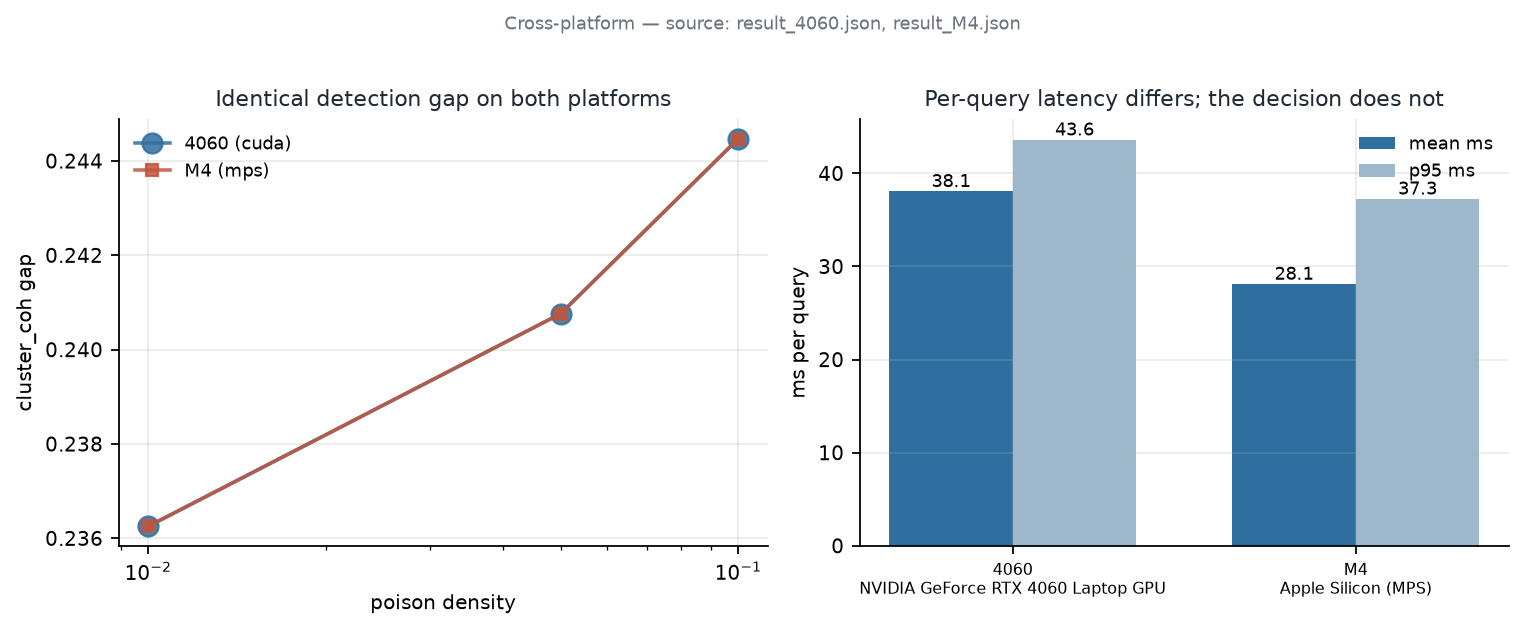
\includegraphics[width=\columnwidth]{docs/figures/cross_platform.png}
\caption{Cross-platform reproduction on the byte-identical, hash-verified corpus. The gap-per-density curves for an RTX~4060 (CUDA) and an Apple~M4 (MPS) are indistinguishable at plot resolution; the platforms differ in latency ($38.1$ vs.\ $28.1$\,ms mean), not in the detection decision.}
\label{fig:xplat}
\end{figure}
Because the detector is byte-frozen and the geometric statistic is deterministic given the
index, its behaviour should not depend on the machine it runs on---and it does not. Rebuilding
the corpus from pinned sources and re-embedding on three platforms across two accelerator
backends---an RTX~5080 and an RTX~4060 (CUDA) and an Apple~M4 (Metal/MPS)---each gated to the
identical order-sensitive SHA-256 corpus hash and per-document fingerprint, the poison--clean
gap, its SNR, and $0\%$ templated poison-evasion reproduce on every platform, density, and seed;
the two independently re-embedded external machines agree on the gap to within $5\times10^{-7}$,
several cells bit-identical. The separation is a property of the attack's
geometry, not of one GPU's manifold or one vendor's kernels---a degree of reproducibility
uncommon in poisoning-defence evaluations, which we report as a first-class result.

The detector is also cheap: it adds a single threshold comparison against a precomputed, cached
statistic, so detection cost is dominated by the retrieval the RAG system already performs.
End-to-end per-query latency is $13$--$38$\,ms mean (p95 $\le 44$\,ms) across the three platforms, with no LLM call and no external API; the FAISS HNSW index makes
neighbour lookups $O(\log N)$, so per-query cost is effectively flat as the corpus grows.

\subsection{Validation at Million-Document Scale}
\label{subsec:scale}
The deployment argument rests on detection cost staying flat as the corpus grows; we
measure that directly at $N=1{,}000{,}000$ documents---ten times the primary corpus,
and the largest scale we run. Per-query latency is $15.0$\,ms mean ($18.2$\,ms p95),
of which the cluster-coherence retrieval and gate check are $\approx\!0.4$\,ms; the
remainder is the encoder forward pass, which is independent of corpus size. The
detector's own cost therefore stays \emph{sub-millisecond} at a million
documents---a ten-fold corpus increase moves the retrieval-plus-gate term by a
fraction of a millisecond---confirming the $O(\log N)$ deployment claim by measurement
rather than extrapolation. Detection holds at scale: the
poison--clean gap is density-invariant ($+0.245$ at $1\%$, $+0.249$ at $5\%$) at an
SNR near $5.6$, poison-evasion is $0\%$ on every condition and seed, and the
non-oracle document-FPR is $0.70\%$---a $0.011\%$ deviation from the $0.69\%$
target.

Three scope notes accompany it. \emph{(i)~A broader corpus.} The security-only source does not
reach a million deduplicated documents, so the $1$M corpus draws from ten technical Stack
Exchange sites---genuinely in-domain technical text, a \emph{distinct, larger} corpus from that
of \S\ref{subsec:eff} and not out-of-domain padding, so the result generalizes to a broader
corpus at scale rather than enlarging the same one. \emph{(ii)~Densities run.} The deterministic
poison budget fills $1\%$ and $5\%$ at this $N$; $10\%$ ($P=100{,}000$) exceeds it and was left
unrun rather than fabricated, density-invariance across the full band being established at
$100{,}000$ (\S\ref{subsec:geom}). \emph{(iii)~Calibration.} The $1$M point extends the trend to
three scales---deviation $0.075\%$, $0.016\%$, $0.011\%$---shrinking as Observation~2 implies;
because it uses the broader corpus we read it as direction, not a fitted exponent.

\section{Discussion}

\subsection{Deployment Implications}
SEVA's operating envelope is its central practical contribution: detection is a single
threshold comparison against a precomputed corpus statistic---no LLM call, no external API, no
cryptographic registration, $13$--$38$\,ms per query with identical detection across CUDA and
Apple-Silicon backends, and a retrieval-plus-gate cost that stays sub-millisecond at a million
documents (\S\ref{subsec:scale}). This is the envelope local, offline RAG on personal and edge
hardware requires and that certified, decoder-access, and provenance-based defenses cannot
meet. The signal is also \emph{corpus-level}: cluster coherence is computed once over the whole
corpus and cached, so it sees the injected cluster even when only one of its passages is
retrieved---a view a per-query filter structurally cannot reconstruct. This suits on-device,
air-gapped, and no-egress deployments alike: the only standing cost is the corpus-level
precompute, and re-screening after an ingestion batch touches only the new documents and their
neighbourhoods.

\subsection{What Cluster Coherence Adds Over Deduplication}
Cluster coherence is a group-cohesion signal, not the pairwise near-duplicate score a
deduplicator computes---and that difference is what the cross-domain results expose. Averaging
similarity over a $K$-neighbour group rather than a single nearest neighbour, it reads the
multi-passage \emph{cluster} an injection forms, giving it two properties a pairwise method
lacks: a separation invariant to how large that cluster grows (Table~\ref{tab:coh}), and
detection of a passage even when no clean document is its near-twin. Against lexical
filtering---PoisonedRAG's own tested defense---this is decisive: corpus-fragile filtering fails
where benign duplication is high while cluster coherence holds. Against embedding deduplication
it is an honest edge, not a rout: $s_{nd}$ is competitive, with cluster coherence's advantage
clearest where benign redundancy is moderate (Natural Questions) and at parity where it is very
sparse or very dense---we claim the former and disclose the latter.

\subsection{What the Geometry Does and Does Not Buy}
The gate fires on one property---that the passages injected for a target occupy a tight
neighbourhood in embedding space---so evading it means injecting poison that does \emph{not}
cluster. Attacks that preserve the shared-recipe structure cannot do this: a diversity-injection
adversary that spreads poison across semantic frames, perturbing each passage to lower its
cohesion, reduces poison cohesion only marginally and leaves every injected passage above the
gate ($0\%$ poison-evasion). Within that family the geometry is decisive, and it is decisive for
a reason the soft signals never had: cohesion is a property of the attack's construction, not of
vocabulary an adversary can normalise away.

What it does \emph{not} buy is a cost floor. Dispersion and retrievability can be purchased
together, cheaply, by abandoning the shared recipe (\S\ref{subsec:boundary}), and doing so costs
the adversary nothing measurable---the bypass is more effective end to end than the attack it
replaces. Figure~\ref{fig:frontier} shows why the intuition that it should be expensive is
wrong: payload prominence trades evasion against retrievability, but the adversary's optimum
sits at $25\%$ prominence, where evasion is still total, so the gate never binds at the
operating point a rational attacker chooses. We state this plainly because the opposite claim is
easy to make and we made it ourselves before measuring: a geometric gate raises the bar for the
attack it reads, and does not raise it at all for an attacker willing to write different text.

\section{Limitations}
\label{sec:limits}
SEVA's scope is stated, not stumbled into; the following are the boundaries of the
claimed regime.

\emph{Injections that form no cluster.} The sharpest limitation is measured, not hypothetical
(\S\ref{subsec:boundary}): an adversary who abandons the shared recipe and anchors each injected
passage to a distinct benign host evades the deployed gate on \emph{every} target while $84\%$
of clones remain retrievable, corrupting $26$--$28\%$ of targets end to end---more than the
$18\%$ the templated attack achieves undefended. Neither injection multiplicity nor
nearest-neighbour duplication as a second geometric signal recovers detection, and
single-document injections that mimic the clean distribution~\cite{corruptrag} form no cluster
at all. Reproduced at a matched operating point, CleanBase~\cite{cleanbase} fails on exactly the
same inputs, so this is a property of the mutual-similarity assumption---and of the
cohesion-detection family, not SEVA alone. A defender should read our positive results as
bounded accordingly: the gate eliminates the dominant published attack at negligible cost, and
does not raise the price for an adversary who switches strategy. Closing that gap plausibly
requires a signal that is not purely geometric.

\emph{Calibration assumption.} Like any calibrated detector, SEVA assumes access
to a reference sample of the attack class for threshold setting; we show that a
threshold calibrated on a disjoint reference sample and then frozen generalizes to
held-out poison of the same class at $0\%$ poison-evasion.
We do not claim calibration-free detection.

\emph{Corpus scale.} The $O(\log N)$ deployment claim is now \emph{measured}, not
extrapolated: at $N=1{,}000{,}000$ documents the detector's retrieval-plus-gate cost
stays sub-millisecond and per-query latency stays in the $100{,}000$-document band
($15.0$\,ms), with $0\%$ poison-evasion and on-target calibration
(\S\ref{subsec:scale}). That run uses a broader technical corpus---the security-only
source does not reach a million deduplicated documents---and the deterministic poison
budget fills $1\%$ and $5\%$ contamination there; behaviour beyond a million, and at
$10\%$ contamination at that scale, is the remaining open edge.

\emph{Encoder scope.} The geometric signal is validated across three embedding models
of independent pre-training lineages---bge (BAAI), e5 (Microsoft), and gte (Alibaba),
each under its correct symmetric convention (\S\ref{subsec:encoder})---so it is not an
artifact of one encoder's manifold. The boundary we do \emph{not} claim is invariance
to embeddings adversarially trained or otherwise built to be poison-aware: an encoder
optimized to scatter templated injections away from their own siblings could in
principle flatten the cohesion gap, and we make no claim against that class.

\section{Conclusion}
We presented SEVA, a lightweight, LLM-free detector of templated multi-passage corpus
poisoning built on a single geometric signal operated as a hard gate, and used it to
characterize what cohesion-based detection can and cannot do. In-domain under frozen,
non-oracle calibration it detects the attack at $0\%$ poison-evasion across three seeds at
$0.58\%$ document-FPR, catches PoisonedRAG's own poison at $82$--$98\%$ across three corpora,
and beats the per-query state of the art in a reproduced, matched-FPR head-to-head---at
$13$--$38$\,ms per query, invariant to contamination density, embedding encoder, and hardware
backend, and measured to $10^6$ documents. We also delimit the assumption underlying the whole
cohesion-detection family: host-anchored cloning evades the gate entirely while remaining
retrievable, no complementary geometric signal we tested closes the gap, and the bypass is not
expensive---it corrupts more targets than the attack it replaces. Detecting injections that leave no
duplication footprint, without an LLM in the loop, remains open.

\appendices


\section{Per-Seed Confusion Matrices}
\label{app:confusion}
We report complete confusion counts for every in-domain condition, the per-seed
reporting that the primary results table of the main paper summarizes. Table~\ref{tab:confL1}
gives the L1 (full signal set) matrices: every cell has $\mathrm{FN}=0$---no
templated poison passage evades detection at any density or seed---which is the
basis for the $0\%$ L1 poison-evasion. Table~\ref{tab:confL23} gives L2 and L3, the
ablated composite, where $\mathrm{FN}>0$ is the adaptive collapse the geometric hard
gate (main paper) eliminates. Table~\ref{tab:percond} converts these
counts into per-condition detection rates---poison-evasion with Wilson upper bounds,
and document- and query-level false-positive rates---for all nine conditions.

\begin{table}[t]
\centering
\caption{Complete per-seed confusion matrices at L1 (full signal set), in-domain
Security corpus. Every cell has $\mathrm{FN}=0$: the $0\%$ L1 poison-evasion reported
in the main paper is exact, not rounded.}
\label{tab:confL1}
\begin{tabular}{llcccc}
\toprule
Density & Seed & TP & FN & FP & TN \\
\midrule
\multirow{3}{*}{1\%}  & 42  & 125 & 0 & 15 & 3287 \\
                      & 7   & 125 & 0 & 24 & 3255 \\
                      & 123 & 125 & 0 & 14 & 3222 \\
\midrule
\multirow{3}{*}{5\%}  & 42  & 138 & 0 & 17 & 3244 \\
                      & 7   & 138 & 0 & 27 & 3231 \\
                      & 123 & 138 & 0 & 17 & 3197 \\
\midrule
\multirow{3}{*}{10\%} & 42  & 156 & 0 & 13 & 3202 \\
                      & 7   & 156 & 0 & 22 & 3196 \\
                      & 123 & 156 & 0 & 15 & 3183 \\
\bottomrule
\end{tabular}
\end{table}

\begin{table}[t]
\centering
\caption{Per-seed confusion at L2 and L3 (soft signals ablated), in-domain---the
composite's adaptive collapse. The geometric hard gate (main paper)
recovers $0\%$ poison-evasion on these same conditions.}
\label{tab:confL23}
\begin{tabular}{llcccc}
\toprule
 & & \multicolumn{2}{c}{L2} & \multicolumn{2}{c}{L3} \\
\cmidrule(lr){3-4}\cmidrule(lr){5-6}
Density & Seed & TP & FN & TP & FN \\
\midrule
\multirow{3}{*}{1\%}  & 42  & 71 & 54  & 70 & 55  \\
                      & 7   & 71 & 54  & 76 & 49  \\
                      & 123 & 68 & 57  & 70 & 55  \\
\midrule
\multirow{3}{*}{5\%}  & 42  & 54 & 84  & 54 & 84  \\
                      & 7   & 70 & 68  & 70 & 68  \\
                      & 123 & 54 & 84  & 54 & 84  \\
\midrule
\multirow{3}{*}{10\%} & 42  & 42 & 114 & 42 & 114 \\
                      & 7   & 45 & 111 & 45 & 111 \\
                      & 123 & 42 & 114 & 42 & 114 \\
\bottomrule
\end{tabular}
\end{table}

\begin{table}[t]
\centering
\caption{Per-condition in-domain detection rates---all nine density$\times$seed
conditions, the full breakdown the primary table of the main paper summarizes,
for the full signal set (tier~L1). The evasion column gives the templated-poison
poison-evasion rate with its $95\%$ Wilson upper bound in parentheses, computed from
the per-condition poison-encounter count $n$; Doc-FPR and query-FPR are the
document- and query-level false-positive rates at the $0.69\%$ non-oracle operating
point. Poison-evasion is $0\%$ at every condition (each cell has $\mathrm{FN}=0$,
Table~\ref{tab:confL1}); on the templated attack the deployed geometric hard gate
coincides with the full signal set at $0\%$ poison-evasion, their divergence under adaptation
being the subject of the geometric-core table in the main paper. The grand-mean row averages the nine
conditions ($n=1{,}257$ pooled encounters); the high-encounter row is a dedicated
frozen-gate run ($25{,}000$ templated encounters, $0$ evasions) tightening the
templated-evasion upper bound to $0.0154\%$. All quantities in \%.}
\label{tab:percond}
\begin{tabular}{llrccc}
\toprule
Density & Seed & $n$ & Evasion (95\% Wilson) & Doc-FPR & query-FPR \\
\midrule
\multirow{3}{*}{1\%}  & 42  & 125 & $\mathbf{0.0}$\,(3.0) & 0.45 & 1.88 \\
                      & 7   & 125 & $\mathbf{0.0}$\,(3.0) & 0.73 & 2.75 \\
                      & 123 & 125 & $\mathbf{0.0}$\,(3.0) & 0.43 & 1.75 \\
\midrule
\multirow{3}{*}{5\%}  & 42  & 138 & $\mathbf{0.0}$\,(2.7) & 0.52 & 2.00 \\
                      & 7   & 138 & $\mathbf{0.0}$\,(2.7) & 0.83 & 3.38 \\
                      & 123 & 138 & $\mathbf{0.0}$\,(2.7) & 0.53 & 2.13 \\
\midrule
\multirow{3}{*}{10\%} & 42  & 156 & $\mathbf{0.0}$\,(2.4) & 0.40 & 1.63 \\
                      & 7   & 156 & $\mathbf{0.0}$\,(2.4) & 0.68 & 2.75 \\
                      & 123 & 156 & $\mathbf{0.0}$\,(2.4) & 0.47 & 1.88 \\
\midrule
\multicolumn{2}{l}{Grand mean}    & $1{,}257$  & $\mathbf{0.0}$           & 0.56 & 2.24 \\
\multicolumn{2}{l}{High-enc.\ CI} & $25{,}000$ & $\mathbf{0.0}$\,(0.0154) & ---  & ---  \\
\bottomrule
\end{tabular}
\end{table}

\section{Attack Construction}
\label{app:attack}
\emph{Templated poison (in-domain).} For each target query we inject multiple
passages generated from a shared security-domain template, so the injected set for
a query is internally homogeneous; contamination is swept at $1\%$, $5\%$, and
$10\%$ of the corpus. \emph{Released PoisonedRAG (cross-domain).} We use the attack
authors' published adversarial passages (PoisonedRAG) for Natural Questions
and HotpotQA ($100$ target queries, $5$ passages each), following their released
construction in which each passage prepends the target question to an LLM-crafted
payload satisfying both retrieval and generation objectives; we add no
re-implementation of our own. \emph{Adaptive adversary (L2/L3).} We model the
keyword-dropping adversary by normalizing the soft signals at the feature
level---keyword density at L2, keyword density and sentence-length structure at
L3---without embedding-space optimization---gradient-based methods such as
GCG or AutoDAN---which is the capability the geometric
gate is built to withstand.

\emph{Host-anchored clones (boundary experiment).} For each of the $50$ adversarial target
queries we take the top-ranked benign document, rewrite it with an offline LLM
(\texttt{mistral:7b-instruct}, temperature $0$) to preserve meaning while changing surface form,
and splice the payload after the first sentence, truncating to $300$ words. Detection is
LLM-free throughout; the LLM is used only for attack generation and for the answer-corruption
check, which is judged by an offline generator (\texttt{gpt-oss:20b}, temperature $0$) counting
payload markers in the answer with and without the clone present. A target counts as corrupted
when the poisoned answer contains at least two payload markers and strictly more than the clean
answer does. Cohesion for these clones is measured in the corpus the attack actually creates---
clean documents plus the injected clones, with no templated poison present---since the two
injection strategies are alternatives, not a combination.

\section{Calibration Thresholds and Reproducibility}
\label{app:repro}
Table~\ref{tab:tau} lists the calibrated thresholds. The deployed geometric gate
sits well below poison coherence ($\approx\!0.99$) and above clean
($\approx\!0.75$) on every corpus. All results use BAAI/bge-large-en-v1.5
($1024$-d, $\ell_2$-normalized) with a FAISS HNSW index ($M=32$,
$\mathrm{efConstruction}=200$); cluster coherence uses $K=5$ with
$K_{\mathrm{FETCH}}=20$ over-fetch. In-domain runs use calibration seeds $42$, $7$,
$123$ over $2{,}000$ benign queries split $60/40$ between calibration and
evaluation, at a $0.0069$ false-positive target throughout. Cross-platform
reproduction---identical detection across CUDA and Apple-Silicon backends on this
byte-identical hash-verified corpus---is reported in the main paper.
Per-condition
artifacts (confusion counts, thresholds, latencies) are recorded per seed and
density.

\begin{table}[t]
\centering
\caption{Calibrated thresholds. The geometric gate (deployed) and the composite
tiers (ablation), in-domain ranges shown across $1$--$10\%$ density.}
\label{tab:tau}
\begin{tabular}{lc}
\toprule
Detector / corpus & $\tau$ \\
\midrule
Geometric gate --- Security (in-domain) & $\approx 0.84$ \\
Geometric gate --- Natural Questions    & $0.832$ \\
Geometric gate --- HotpotQA             & $0.804$ \\
Composite L1 --- Security ($1\%\!\to\!10\%$) & $0.58 \to 0.64$ \\
Composite L2 --- Security               & $0.67 \to 0.77$ \\
Composite L3 --- Security               & $0.69 \to 0.77$ \\
\bottomrule
\end{tabular}
\end{table}

\section{Defense Capability Comparison}
\label{app:compare}
Table~\ref{tab:caps} positions SEVA against the defenses PoisonedRAG and its
successors evaluate, by deployment capability rather than by lifted attack-success
numbers (which the head-to-head of the main paper replaces with a
reproduced measurement). SEVA is the only entry that is simultaneously LLM-free,
decoder-free, registration-free, corpus-level, and evaluated across the $1$--$10\%$
density band.

\begin{table}[t]
\centering
\caption{Deployment-capability comparison (factual properties of each defense, per
its publication; not lifted ASR numbers). $\checkmark$ = property held.}
\label{tab:caps}
\begin{tabular}{lccccc}
\toprule
Defense & \rotatebox{90}{LLM-free\,} & \rotatebox{90}{No decoder\,} &
\rotatebox{90}{No pre-reg.\,} & \rotatebox{90}{Corpus-level\,} & Density \\
\midrule
RobustRAG    & $\times$\,($5\times$) & $\checkmark$ & $\checkmark$ & $\times$ & $\sim$0.001\% \\
AV Filter    & $\times$ & $\times$ & $\checkmark$ & $\times$ & $\sim$0.001\% \\
RAGShield    & $\checkmark$ & $\checkmark$ & $\times$ & --- & $\sim$0.001\% \\
RAGDefender  & $\checkmark$ & $\checkmark$ & $\checkmark$ & $\times$ & $\sim$1\% \\
\textbf{SEVA (ours)}          & $\checkmark$ & $\checkmark$ & $\checkmark$ & $\checkmark$ & \textbf{1--10\%} \\
\bottomrule
\end{tabular}
\end{table}

\section{Supporting Detection Tables}
\label{app:tables}
Table~\ref{tab:roc} reports the matched-FPR catch-rate sweep underlying the
corpus-fragility result (main paper, ``Lexical Duplicate Filtering Is Corpus-Fragile''):
the headline operating-point numbers appear in the main paper's cross-domain table, and
the sweep here shows lexical filtering catching nothing below a $2\%$ false-positive rate
while cluster coherence catches the attack at the $0.69\%$ operating point. Table~\ref{tab:agg}
reports the per-query aggregation that, by requiring $\geq\!2$ flagged documents per query,
cuts the benign query-level false-positive rate $3.5\times$ at no cost to catch rate.

\begin{table}[t]
\centering
\caption{Matched-FPR catch rate of the released PoisonedRAG attack on Natural
Questions and HotpotQA as the operating false-positive rate is swept, for cluster
coherence (ours), lexical MinHash, and embedding $s_{nd}$. Lexical filtering catches
nothing on these duplicate-rich benchmarks at any deployable FPR below $2\%$; cluster coherence
catches the attack at the $0.69\%$ operating point on both.}
\label{tab:roc}
\begin{tabular}{llccc}
\toprule
Corpus & FPR & \texttt{cluster\_coh} & MinHash & $s_{nd}$ \\
\midrule
\multirow{4}{*}{Natural Questions}
 & 0.5\%  & 70\% & 0\%   & 30\% \\
 & 0.69\% & \textbf{82\%} & 0\% & 52\% \\
 & 1\%    & 92\% & 0\%   & 74\% \\
 & 2\%    & 98\% & 100\% & 95\% \\
\midrule
\multirow{4}{*}{HotpotQA}
 & 0.5\%  & 95\%  & 0\% & 97\% \\
 & 0.69\% & \textbf{97\%} & 0\% & 98\% \\
 & 1\%    & 100\% & 0\% & 99\% \\
 & 2\%    & 100\% & 0\% & 100\% \\
\bottomrule
\end{tabular}
\end{table}

\begin{table}[t]
\centering
\caption{Per-query aggregation on the PoisonedRAG corpus (same $0.69\%$ document
threshold). Requiring $\geq\!2$ flagged documents per query exploits the attack's
multi-passage structure to cut the benign query-level false-positive rate
$3.5\times$ at no cost to catch rate.}
\label{tab:agg}
\begin{tabular}{lcc}
\toprule
Aggregation rule & Benign query-FPR & Poison catch \\
\midrule
$\geq\!1$ flagged & 3.15\% & 98.0\% \\
$\geq\!2$ flagged & \textbf{0.90\%} & \textbf{98.0\%} \\
\bottomrule
\end{tabular}
\end{table}

\section{Signal Inventory (Composite Ablation)}
\label{app:signals}
Table~\ref{tab:signals} is the ten-signal inventory underlying the composite ablation of the
main paper: only cluster coherence combines a high in-domain SNR with robustness to both the
domain-confound control and adaptive normalization.

\begin{table}[t]
\centering
\caption{In-domain signal inventory (Security Stack Exchange, seed~42, $1\%$
density). Only cluster coherence combines a high SNR with robustness to both the
domain-confound control and adaptive normalization; the soft signals are weak
in-domain, and the strongest of them (keyword density) is both confounded
(SNR~$38.4\!\to\!8.1$ against a general-domain corpus) and adversary-normalizable.
SEVA deploys the geometric signal alone; the rest are the ablation.}
\label{tab:signals}
\setlength{\tabcolsep}{4pt}
\begin{tabular}{llc>{\raggedright\arraybackslash}p{2.1cm}}
\toprule
Signal & Type & In-domain SNR & Status \\
\midrule
\texttt{cluster\_coh}  & geometric  & $5.99$  & \textbf{deployed} \\
\texttt{kw\_density}   & keyword    & $8.10$  & confounded, normalizable (L2) \\
\texttt{sent\_unif}    & structural & $1.40$  & ablated \\
\texttt{topic\_drift}  & semantic   & $1.18$  & ablated \\
\texttt{punct}         & structural & $1.04$  & ablated \\
\texttt{doc\_length}   & structural & $0.92$  & ablated \\
\texttt{avg\_sent\_len} & structural & $0.53$  & normalizable (L3) \\
\texttt{content\_ttr}  & lexical    & $-1.09$ & ablated \\
\texttt{ttr}           & lexical    & $-1.12$ & ablated \\
\texttt{repeat\_rate}  & lexical    & $-0.48$ & excluded \\
\bottomrule
\end{tabular}
\end{table}

\section{Geometric Core vs.\ Composite}
\label{app:core}
Table~\ref{tab:core} accompanies the geometric-core discussion of the main paper: the composite
matches the hard gate on the naive attack, dilutes detection on real PoisonedRAG, and collapses
under the keyword-dropping adversary, while the hard gate holds.

\begin{table}[t]
\centering
\caption{The geometric core vs.\ the multi-signal composite (the ablation), at
$0.69\%$ non-oracle document-FPR, by poison-evasion rate (lower is better). The
composite equals the hard gate on the naive attack, but the soft signals dilute
detection on real PoisonedRAG and collapse under the keyword-dropping adversary,
while the geometric hard gate holds.}
\label{tab:core}
\begin{tabular}{lcc}
\toprule
\multirow{2}{*}{Attack} & \texttt{cluster\_coh} & 10-signal \\
       & hard gate & composite \\
\midrule
Templated (held-out)    & \textbf{0\%} & 0\% \\
Real PoisonedRAG        & \textbf{2\%} & 28\% \\
Adaptive (keyword-drop) & \textbf{0\%} & 49--57\% \\
\bottomrule
\end{tabular}
\end{table}

\section{Cross-Platform Reproduction}
\label{app:xplat}
Per-platform detail for the cross-platform reproduction reported in the main paper: identical detection across CUDA and Apple-Silicon backends on the byte-identical hash-verified corpus.

\begin{table}[t]
\centering
\caption{Cross-platform reproduction on a byte-identical, hash-verified corpus (SHA-256
\texttt{28ec3811}$\dots$): \emph{identical} detection across CUDA and Apple-Silicon
backends---the gap, SNR, and $0\%$ templated poison-evasion match on every platform,
density, and seed (the two re-embedded external machines agree on the gap to within
$5\times10^{-7}$)---at $13$--$38$\,ms per query.}
\label{tab:xplat}
\begin{tabular}{llcccc}
\toprule
Platform & Backend & Gap ($1$--$10\%$) & SNR & Templ.\ evasion & Latency mean/p95 \\
\midrule
RTX 5080 (desktop) & CUDA & $+0.236$ to $+0.245$ & $5.9$--$6.1$ & $\mathbf{0\%}$ & $13.4$--$15.7$\,/\,$\le\!18.8$\,ms \\
RTX 4060 (laptop) & CUDA & $+0.236$ to $+0.245$ & $5.9$--$6.1$ & $\mathbf{0\%}$ & $38.1$\,/\,$43.6$\,ms \\
Apple M4 (laptop) & MPS & $+0.236$ to $+0.245$ & $5.9$--$6.1$ & $\mathbf{0\%}$ & $28.1$\,/\,$37.3$\,ms \\
\bottomrule
\end{tabular}
\end{table}

\section{Encoder-Invariance Detail}
\label{app:encoder}
Per-encoder detail for Observation~3 of the main paper: the geometric gate under three embedding lineages on the identical hash-verified in-domain corpus, each calibrated non-oracle in its correct symmetric convention.

\begin{table}[t]
\centering
\caption{Encoder-invariance: the geometric gate across three embedding lineages on the
identical hash-verified in-domain corpus, each calibrated non-oracle in its correct
symmetric convention. Templated poison-evasion is $0\%$ for all three; the absolute gap
shrinks only as the clean manifold concentrates (clean coherence $0.751\!\to\!0.881$),
while the scale-normalized SNR holds. Values span $1$--$10\%$ density.}
\label{tab:encoder}
\begin{tabular}{llccccc}
\toprule
Encoder & Lineage & Clean coh. & Poison coh. & Gap & SNR & Templ.\ evasion \\
\midrule
bge-large   & BAAI      & $0.751$ & $0.990$ & $+0.236$ to $+0.245$ & $5.9$--$6.1$ & $\mathbf{0\%}$ \\
e5-large-v2 & Microsoft & $0.866$ & $0.990$ & $+0.122$ to $+0.127$ & $6.4$--$6.7$ & $\mathbf{0\%}$ \\
gte-large   & Alibaba   & $0.881$ & $0.996$ & $+0.113$ to $+0.117$ & $5.2$--$5.3$ & $\mathbf{0\%}$ \\
\bottomrule
\end{tabular}
\end{table}

\section{Reproduced Head-to-Head Detail}
\label{app:h2h}
Per-defense detail for the reproduced, shared-corpus, matched-FPR head-to-head of the main paper.

\begin{table}[t]
\centering
\caption{Reproduced head-to-head against the per-query state of the art on a
shared Security corpus and templated attack. RAGDefender uses SEVA's encoder
(bge-large), isolating the algorithmic difference; its native filter has no
no-attack gate and removes half of all clean documents, so the catch comparison
is made at a matched $\sim$0.8\% benign-FPR operating point (looser than SEVA's own
$\sim$0.6\%) using a best-case idealized threshold in RAGDefender's favour.}
\label{tab:h2h}
\begin{tabular}{lcc}
\toprule
\multirow{2}{*}{Defense} & Templated catch & Native benign \\
        & @ matched $\sim$0.8\% FPR & doc-FPR \\
\midrule
SEVA & \textbf{100\%} & $\sim$0.6\% \\
RAGDefender & $\sim$89\% & 50.4\% \\
\bottomrule
\end{tabular}
\end{table}

\section{Million-Document Scale Detail}
\label{app:scale}
Per-density detail for the million-document scale validation reported in the main paper.

\begin{table}[t]
\centering
\caption{Validation at million-document scale: $N=1{,}000{,}000$, a broader hash-gated
technical corpus (SHA-256 \texttt{317eb43c}$\dots$---\emph{distinct} from the
cross-platform corpus of the main paper). Latency is $15.0$\,ms mean / $18.2$\,ms p95,
of which retrieval and gate are $\approx\!0.4$\,ms (sub-millisecond at $10\times$ scale);
poison-evasion is $0\%$, the gap density-invariant, and the non-oracle document-FPR
$0.70\%$. The poison budget fills $1\%$ and $5\%$; $10\%$ exceeds it. Three seeds.}
\label{tab:scale}
\begin{tabular}{lccccc}
\toprule
Density & $n_{\mathrm{poison}}$ & Gap & SNR & Evasion & Doc-FPR \\
\midrule
$1\%$ & $10{,}000$ & $+0.245$ & $5.63$ & $\mathbf{0\%}$ & $0.68\%$ \\
$5\%$ & $50{,}000$ & $+0.249$ & $5.57$ & $\mathbf{0\%}$ & $0.72\%$ \\
\bottomrule
\end{tabular}
\end{table}

\section{Cross-Domain Detection Detail}
\label{app:xdomain}
Per-corpus detail for the cross-domain results reported in the main paper: cluster coherence against lexical MinHash and embedding near-duplicate detection at the matched non-oracle operating point.

\begin{table}[t]
\centering
\caption{Cross-domain detection of the PoisonedRAG attack at the $0.69\%$ non-oracle
operating point (released poison on Natural Questions and HotpotQA; a faithful black-box
build on Security). \texttt{cluster\_coh} catches the attack on all three corpora
(``Evasion'' is the residual it misses, a detection metric); lexical MinHash filtering is
corpus-fragile, while embedding deduplication ($s_{nd}$) is competitive. ``Benign dup.''\
is the fraction of clean documents sharing a 5-gram.}
\label{tab:xdomain}
\resizebox{\columnwidth}{!}{%
\begin{tabular}{lccccc}
\toprule
\multirow{2}{*}{Corpus} & Benign & \texttt{cluster\_coh} & MinHash & $s_{nd}$ & Poison \\
       & dup. & (ours) & (lexical) & (embed.) & evasion \\
\midrule
Security SE       & 0.24\% & \textbf{98\%} & 98\% & 98\% & 2\% \\
Natural Questions & 1.15\% & \textbf{82\%} & 0\%  & 52\% & 18\% \\
HotpotQA          & 9.06\% & \textbf{97\%} & 0\%  & 98\% & 3\% \\
\bottomrule
\end{tabular}}
\end{table}




\begin{figure}[t]
\centering
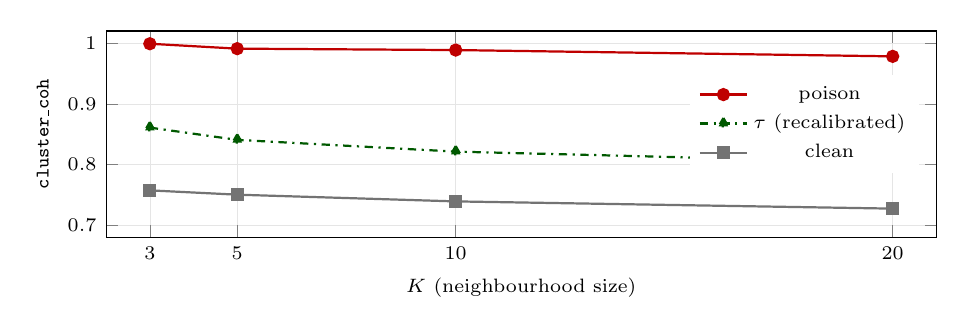
\begin{tikzpicture}
\begin{axis}[width=\columnwidth, height=4.2cm,
  xlabel={$K$ (neighbourhood size)}, ylabel={\texttt{cluster\_coh}},
  xmin=2, xmax=21, ymin=0.68, ymax=1.02, xtick={3,5,10,20},
  tick label style={font=\scriptsize}, label style={font=\scriptsize},
  legend style={font=\scriptsize, at={(0.98,0.55)}, anchor=east, draw=none},
  grid=both, grid style={line width=.2pt, draw=gray!20}]
\addplot[thick, red!75!black, mark=*] coordinates {(3,0.9990) (5,0.9909) (10,0.9886) (20,0.9782)};
\addlegendentry{poison}
\addplot[thick, green!35!black, dash dot, mark=triangle*] coordinates {(3,0.8607) (5,0.8405) (10,0.8211) (20,0.8032)};
\addlegendentry{$\tau$ (recalibrated)}
\addplot[thick, black!55, mark=square*] coordinates {(3,0.7572) (5,0.7501) (10,0.7390) (20,0.7271)};
\addlegendentry{clean}
\end{axis}
\end{tikzpicture}
\caption{The separation is not an artifact of $K=5$. Increasing $K$ lowers clean, poison and the
recalibrated threshold together, leaving the margin intact: catch is $100\%$ at every value
(Table~\ref{tab:ksens}).}
\label{fig:ksens}
\end{figure}

\section{Complete Sensitivity Measurements}
\label{app:sens}
The main text summarizes these; the full sweeps are below. Every row recalibrates the threshold
non-oracle on clean coherence alone, so no row borrows information from the poison.

\begin{table}[t]
\centering
\caption{$K$-sensitivity. \texttt{cluster\_coh} recomputed over the whole $100{,}000$-document
corpus for each $K$, with $\tau$ recalibrated at the $0.69\%$ target each time. Detection does
not depend on the frozen choice of $K=5$; that value reproduces the cached \texttt{doc\_coh}
exactly ($|\Delta|=0.00000$).}
\label{tab:ksens}
\begin{tabular}{lccccc}
\toprule
$K$ & $\tau$ & Clean coh. & Poison coh. & Catch & Clean FPR \\
\midrule
$3$  & $0.8607$ & $0.7572$ & $0.9990$ & $\mathbf{100\%}$ & $0.688\%$ \\
$5$  & $0.8405$ & $0.7501$ & $0.9909$ & $\mathbf{100\%}$ & $0.691\%$ \\
$10$ & $0.8211$ & $0.7390$ & $0.9886$ & $\mathbf{100\%}$ & $0.691\%$ \\
$20$ & $0.8032$ & $0.7271$ & $0.9782$ & $\mathbf{100\%}$ & $0.691\%$ \\
\bottomrule
\end{tabular}
\end{table}

\begin{table}[t]
\centering
\caption{Operating-point sweep, in-domain, frozen $K=5$. Catch is $100\%$ at every deployable
false-positive target, including one seven times tighter than the reported operating point.
Rank-based AUC over the clean/poison separation is $0.99994$.}
\label{tab:fprsweep}
\begin{tabular}{lccc}
\toprule
FPR target & $\tau$ & Catch & Realized FPR \\
\midrule
$0.10\%$ & $0.8637$ & $\mathbf{100\%}$ & $0.100\%$ \\
$0.25\%$ & $0.8519$ & $\mathbf{100\%}$ & $0.251\%$ \\
$0.50\%$ & $0.8444$ & $\mathbf{100\%}$ & $0.500\%$ \\
$0.69\%$ & $0.8408$ & $\mathbf{100\%}$ & $0.691\%$ \\
$1.00\%$ & $0.8367$ & $\mathbf{100\%}$ & $1.000\%$ \\
$2.00\%$ & $0.8272$ & $\mathbf{100\%}$ & $2.000\%$ \\
$5.00\%$ & $0.8130$ & $\mathbf{100\%}$ & $5.000\%$ \\
\bottomrule
\end{tabular}
\end{table}


\begin{figure}[t]
\centering
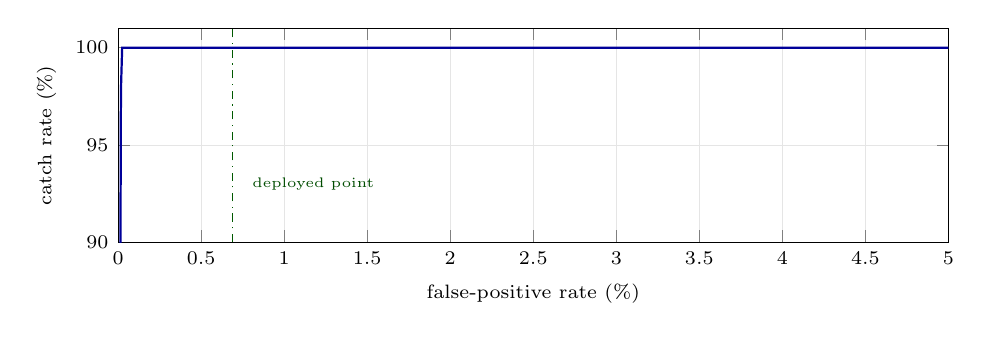
\begin{tikzpicture}
\begin{axis}[width=\columnwidth, height=4.3cm,
  xlabel={false-positive rate (\%)}, ylabel={catch rate (\%)},
  xmin=0, xmax=5, ymin=90, ymax=101,
  tick label style={font=\scriptsize}, label style={font=\scriptsize},
  grid=both, grid style={line width=.2pt, draw=gray!20}]
\addplot[thick, blue!60!black, mark=none] coordinates {(0.0000,0.0200) (0.0000,1.9800) (0.0000,3.9400) (0.0000,5.9200) (0.0011,7.8600) (0.0011,9.8400) (0.0011,11.8000) (0.0011,13.7800) (0.0011,15.7400) (0.0011,17.7200) (0.0021,19.6600) (0.0021,21.6400) (0.0021,23.6000) (0.0021,25.5800) (0.0021,27.5400) (0.0032,29.5000) (0.0032,31.4600) (0.0032,33.4400) (0.0032,35.4000) (0.0032,37.3800) (0.0032,39.3400) (0.0032,41.3000) (0.0032,43.2800) (0.0032,45.2400) (0.0042,47.2000) (0.0042,49.1600) (0.0042,51.1400) (0.0042,53.1000) (0.0053,55.0600) (0.0063,57.0000) (0.0063,58.9800) (0.0063,60.9400) (0.0063,62.9200) (0.0063,64.8800) (0.0084,66.8200) (0.0084,68.7800) (0.0084,70.7600) (0.0095,72.7000) (0.0095,74.6800) (0.0095,76.6400) (0.0105,78.5800) (0.0105,80.5600) (0.0105,82.5200) (0.0116,84.4800) (0.0137,86.4000) (0.0147,88.3600) (0.0147,90.3200) (0.0147,92.3000) (0.0158,94.2400) (0.0158,96.2200) (0.0179,98.1400) (0.0242,100.0000) (0.1274,100.0000) (0.2316,100.0000) (0.3347,100.0000) (0.4389,100.0000) (0.5421,100.0000) (0.6463,100.0000) (0.7495,100.0000) (0.8537,100.0000) (0.9568,100.0000) (1.0600,100.0000) (1.1642,100.0000) (1.2674,100.0000) (1.3716,100.0000) (1.4747,100.0000) (1.5789,100.0000) (1.6821,100.0000) (1.7863,100.0000) (1.8895,100.0000) (1.9937,100.0000) (2.0968,100.0000) (2.2011,100.0000) (2.3042,100.0000) (2.4084,100.0000) (2.5116,100.0000) (2.6158,100.0000) (2.7189,100.0000) (2.8232,100.0000) (2.9263,100.0000) (3.0295,100.0000) (3.1337,100.0000) (3.2368,100.0000) (3.3411,100.0000) (3.4442,100.0000) (3.5484,100.0000) (3.6516,100.0000) (3.7558,100.0000) (3.8589,100.0000) (3.9632,100.0000) (4.0663,100.0000) (4.1705,100.0000) (4.2737,100.0000) (4.3779,100.0000) (4.4811,100.0000) (4.5853,100.0000) (4.6884,100.0000) (4.7926,100.0000) (4.8958,100.0000) (5.0000,100.0000)};
\draw[green!35!black, dash dot] (axis cs:0.69,90) -- (axis cs:0.69,101);
\node[green!30!black, font=\tiny, anchor=west] at (axis cs:0.75,93) {deployed point};
\end{axis}
\end{tikzpicture}
\caption{In-domain ROC over the deployable region, frozen $K=5$. Catch is saturated at $100\%$
well below the operating point; rank-based AUC over the full range is $0.99994$. The $0.69\%$
target is not a tuned optimum---any threshold in this region gives the same detection.}
\label{fig:roc}
\end{figure}

\section{The Boundary in Full}
\label{app:boundaryfull}

\begin{table}[t]
\centering
\caption{Injection multiplicity does not restore detection. Host-anchored clones scored in the
corpus the attack creates ($95{,}000$ clean documents plus the injected clones, no templated
poison present), with both thresholds recalibrated per configuration at the same $0.69\%$
budget. Cohesion rises with multiplicity but stays under $\tau=0.840$ on average.}
\label{tab:multiplicity}
\begin{tabular}{lccccc}
\toprule
Clones/target & Clone coh. & \texttt{cluster\_coh} & $s_{nd}$ & Union gate \\
\midrule
$1$ & $0.722$ & $0\%$    & $20.0\%$ & $13.3\%$ \\
$2$ & $0.746$ & $0\%$    & $13.3\%$ & $6.7\%$  \\
$3$ & $0.772$ & $11.1\%$ & $13.3\%$ & $20.0\%$ \\
$5$ & $0.790$ & $22.7\%$ & $18.7\%$ & $33.3\%$ \\
\bottomrule
\end{tabular}
\end{table}

\begin{table}[t]
\centering
\caption{The payload-prominence frontier with its potency axis (the data behind
Fig.~\ref{fig:frontier}). ``Cands.''\ counts targets whose clone both evades the gate and is
retrieved; flip is the fraction of those whose answer is corrupted; ASR is over all $50$
targets. End-to-end success peaks at $25\%$ payload, where evasion is still total---so the gate
does not bind at the adversary's optimum.}
\label{tab:frontier}
\begin{tabular}{lcccccc}
\toprule
Payload & Coh. & Evades & Retr. & Cands. & Flip & ASR \\
\midrule
$12\%$ & $0.752$ & $100\%$ & $90\%$ & $45$ & $17.8\%$ & $16.0\%$ \\
$25\%$ & $0.764$ & $100\%$ & $78\%$ & $39$ & $35.9\%$ & $\mathbf{28.0\%}$ \\
$37\%$ & $0.777$ & $86\%$  & $72\%$ & $33$ & $33.3\%$ & $22.0\%$ \\
$62\%$ & $0.837$ & $46\%$  & $38\%$ & $13$ & $46.2\%$ & $12.0\%$ \\
\bottomrule
\end{tabular}
\end{table}

\emph{CleanBase reproduction.} We implement the described algorithm directly: an edge joins two
documents when their cosine similarity exceeds $\mu + z\sigma$ of the clean similarity
distribution, and a document is flagged when it belongs to a clique of size $\ge 3$. Rather than
adopt the paper's suggested $z$, we sweep $z$ by bisection until the \emph{clean} false-positive
rate matches our own $0.69\%$ operating point, which lands at $z=2.24$ ($\tau=0.8605$,
realized FPR $0.689\%$)---close to the value the paper suggests, and a comparison neither method
is advantaged by. On templated poison it flags every injected passage; on host-anchored clones
it flags none. Detection is corpus-level and LLM-free for both methods, and both run on the same
cached embeddings, so the comparison isolates the statistic computed from the shared assumption.


\begin{figure}[t]
\centering
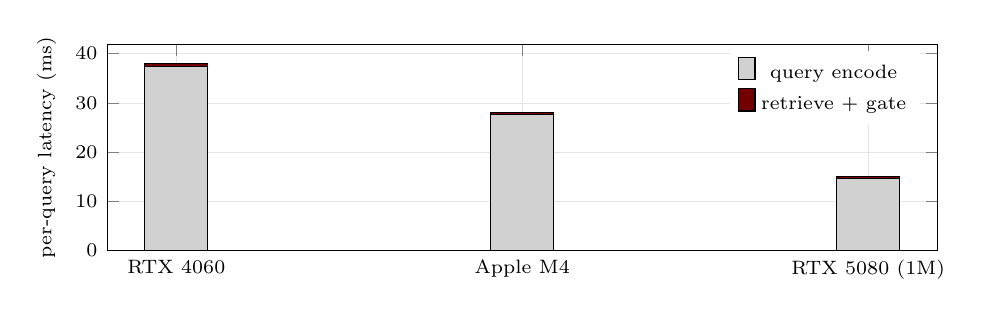
\begin{tikzpicture}
\begin{axis}[width=\columnwidth, height=4.2cm,
  ybar stacked, bar width=8mm,
  symbolic x coords={RTX~4060,Apple~M4,RTX~5080~(1M)},
  xtick=data, ymin=0, ylabel={per-query latency (ms)},
  tick label style={font=\scriptsize}, label style={font=\scriptsize},
  legend style={font=\scriptsize, at={(0.98,0.97)}, anchor=north east, draw=none},
  grid=both, grid style={line width=.2pt, draw=gray!20}]
\addplot[fill=black!18] coordinates {(RTX~4060,37.36) (Apple~M4,27.70) (RTX~5080~(1M),14.61)};
\addlegendentry{query encode}
\addplot[fill=red!45!black] coordinates {(RTX~4060,0.71) (Apple~M4,0.41) (RTX~5080~(1M),0.42)};
\addlegendentry{retrieve $+$ gate}
\end{axis}
\end{tikzpicture}
\caption{Where the per-query millisecond goes. The detector's own contribution---retrieval plus
the threshold test---is $0.41$--$0.71$\,ms on every platform, including at $N=10^6$; the rest is
the encoder forward pass a RAG system already pays. This is why the deployment envelope is
insensitive to corpus size.}
\label{fig:latency}
\end{figure}

\section{Deployment Cost of the Corpus-Level Precompute}
\label{app:cost}
Per-query latency is only half the deployment question; the other half is the one-time
corpus-level pass, which we report rather than amortize away. On the RTX~5080, embedding
$200{,}000$ documents takes $1557$\,s, one HNSW build over that set $259$\,s, and one $K=5$
coherence pass $286$\,s. At $N=10^6$ the measured run required $\approx 7785$\,s to embed and
$\approx 3086$\,s per contamination density for the index and coherence pass, for a total
wall-clock of $3.3$\,h including corpus construction and hash gating. Embedding dominates and is
linear in $N$; the index and coherence terms grow as $N\log N$. Two properties matter
operationally. The pass is incremental: re-screening after an ingestion batch touches only the
new documents and the neighbourhoods they perturb, not the whole corpus. And it is offline: no
query is blocked on it, since detection at query time is a lookup against the cached statistic.

\section{Negative Results, and One Retraction}
\label{app:negative}
Page limits usually push results like these out of a paper. We keep them because the boundary of
\S\ref{subsec:boundary} was only found by running them, and because a reader deciding whether to
deploy a cohesion gate needs them more than another confirmatory table.

\emph{Density-invariance fails on small corpora.} Observation~1 is stated over the evaluated
$1$--$10\%$ range at $N=10^5$, and it holds there. It does \emph{not} hold at $N=10^4$: the
coherence gap collapses to $0.141$ at $1\%$ contamination, and the corresponding run records both
\texttt{gap\_density\_invariant: false} and \texttt{templated\_asr\_zero: false}. The mechanism is
the one Observation~1 relies on read in reverse---with $10^4$ documents and $1\%$ contamination
there are too few injected siblings for a poison passage's $K=5$ neighbourhood to be dominated by
its own cluster. Density-invariance is a large-corpus property. Figure~\ref{fig:scaling} plots
the failure rather than cropping it.

\emph{A complementary signal that did not work.} Host-anchored clones evade cohesion because each
is anchored to a distinct benign host; the natural repair is to add nearest-neighbour duplication
$s_{nd}$, which should spike precisely because a clone stays close to the host it mimics. We
expected this to close the gap. It does not: paraphrasing moves the clone far enough from its
host that $s_{nd}$ stays inside the clean band, catching $13$--$20\%$ of clones, and a union gate
over both signals jointly calibrated to the same budget reaches only $6.7$--$33.3\%$
(Table~\ref{tab:multiplicity}). We report the failed repair because it is what elevates the
finding from ``our statistic has a blind spot'' to ``the geometric information available to this
family does not separate host-anchored clones from their hosts.''

\emph{A retracted claim.} An earlier version of this work argued that evading the gate is
expensive---that dispersion and retrievability could not be bought together, and that the
geometry therefore imposed a cost-of-attack floor. Three separate measurements contradicted it.
The best-case geometric probe found no such necessity; the prominence sweep showed dispersion and
retrievability \emph{are} jointly purchasable at low payload; and, measured on one protocol with
one generator and one corruption criterion, the bypass corrupts $26$--$28\%$ of targets against
$18\%$ for the templated attack it replaces---it is more effective, not less. The earlier claim
survived as long as it did because it compared our figure against a number reported elsewhere
under a different generator, corpus and criterion. We state the correction plainly here: a
cohesion gate raises the bar for the attack it reads and does not raise it for an adversary
willing to write different text.


\section{Corpora, Constants, and Environment}
\label{app:setup}

\begin{table}[t]
\centering
\caption{Evaluation corpora. Benign duplication is the fraction of clean documents sharing a
$5$-gram with another, the property that separates lexical from semantic detection.}
\label{tab:corpora}
\setlength{\tabcolsep}{4pt}
\begin{tabular}{lrccl}
\toprule
Corpus & Docs & Benign dup. & Clean coh. & Role \\
\midrule
Security SE      & $100{,}000$   & $0.24\%$ & $0.750$ & in-domain control \\
Natural Questions& $\approx\!150$k & $1.15\%$ & --- & released poison \\
HotpotQA         & $\approx\!150$k & $9.06\%$ & --- & released poison \\
Multi-site SE    & $1{,}000{,}000$ & --- & $0.748$ & scale \\
\bottomrule
\end{tabular}
\end{table}

\begin{table}[t]
\centering
\caption{Frozen detector constants. No value is tuned per corpus, per density, or per encoder;
$K$ and the operating point are swept only as sensitivity analyses
(Tables~\ref{tab:ksens},~\ref{tab:fprsweep}).}
\label{tab:constants}
\setlength{\tabcolsep}{4pt}
\begin{tabular}{lll}
\toprule
Symbol & Value & Meaning \\
\midrule
$K$ & $5$ & neighbours scored for cohesion \\
$K_{\mathrm{FETCH}}$ & $20$ & over-fetch before rerank \\
$m$ & $1024$ & embedding dimension \\
$M$ / efC & $32$ / $200$ & HNSW graph parameters \\
$\mathrm{FPR}_{\mathrm{TARGET}}$ & $0.0069$ & non-oracle calibration target \\
$k$ & $2$ & flags required per query \\
seeds & $42,7,123$ & calibration partitions \\
\bottomrule
\end{tabular}
\end{table}

\begin{table}[t]
\centering
\caption{Software environment per platform. Detection agrees to $<5\times10^{-7}$ across these
despite different Python, PyTorch, FAISS and sentence-transformers builds---the decision is a
property of the geometry, not of a toolchain.}
\label{tab:env}
\setlength{\tabcolsep}{3.5pt}
\begin{tabular}{llll}
\toprule
 & RTX 5080 & RTX 4060 & Apple M4 \\
\midrule
Python  & $3.11.15$ & $3.13.7$ & $3.11.9$ \\
PyTorch & $2.11.0$+cu128 & $2.6.0$+cu124 & $2.11.0$ \\
Backend & CUDA & CUDA & MPS \\
FAISS   & $1.7.4$ & $1.13.2$ & $1.13.2$ \\
S-T     & $3.0.1$ & $5.3.0$ & $5.2.2$ \\
\bottomrule
\end{tabular}
\end{table}

\section{Deployment Guidance}
\label{app:guidance}
Our results support a narrow recommendation, and we state its limits with it. A cohesion gate is
worth deploying where the threat is the published templated attack: it costs one offline pass and
sub-millisecond per query, needs no LLM, no decoder access and no registration authority, holds
its operating point across encoders and hardware, and---measured end to end---removes all of the
answer corruption that attack produces. For an operator whose realistic adversary is an
opportunistic injector reusing published tooling, that is a favourable trade.

It should not be deployed as though it bounded the adversary. An attacker who reads this paper can
evade it with one paraphrase per target and lose nothing in effectiveness. A gate of this family
is therefore a filter for known attack structure, not a security boundary, and it should sit
behind controls that do not depend on the attacker's text: provenance on the ingestion path,
rate and origin limits on who may write to the corpus, and review of documents that enter through
low-trust channels. The geometric signal tells you when someone has used the standard attack; it
cannot tell you that nobody has attacked.

\section{What Would Close the Boundary}
\label{app:future}
The blind spot is informative about what a repair must do. Host-anchored clones defeat cohesion
because they are, geometrically, ordinary documents: they sit where a benign document sits,
because they were built from one. Any statistic computed \emph{only} from the corpus embedding
geometry therefore has no signal to read---which our failed $s_{nd}$ repair demonstrates rather
than assumes. Three directions do not share that limitation. Provenance breaks the symmetry
without looking at content at all, at the cost of an authority the offline setting was chosen to
avoid. Cross-encoder or entailment scoring between a passage and the claim it supports reads
meaning rather than position, and would see that a clone's payload contradicts its host's own
content; it costs a second model, though not necessarily a generative one. Retrieval-time
consistency---asking whether the documents retrieved for one query agree with each other---is
what the per-query filters already approximate, and pairing it with a corpus-level statistic is
the obvious hybrid our results argue for, since the two fail on disjoint inputs.

\section{Ethics and Responsible Disclosure}
\label{app:ethics}
This work evaluates a defense, but the boundary we report is an attack technique, and we describe
it in enough detail to reproduce. We judged disclosure appropriate on three grounds. The
construction is not novel or difficult---it is copy, paraphrase, splice, and requires no gradient
access, no optimization and no model internals; an adversary willing to spend one LLM call per
target would find it. It defeats a defense family that is being actively proposed for deployment,
so operators need it to calibrate what they are buying. And withholding it would leave our own
positive results overstated, which is the failure mode this paper exists to correct. No live
system was attacked: every experiment runs on a locally constructed corpus with synthetic
payloads, and the released artifacts contain no real credentials or personal data.

\bibliographystyle{IEEEtran}
\begin{thebibliography}{99}
\bibitem{poisonedrag} W. Zou, R. Geng, B. Wang, and J. Jia, ``PoisonedRAG: Knowledge corruption attacks to retrieval-augmented generation of large language models,'' in \emph{Proc. 34th USENIX Security Symposium}, 2025.
\bibitem{avfilter} S. Choudhary, N. Palumbo, A. Hooda \emph{et al.}, ``Through the stealth lens: Rethinking attacks and defenses in RAG,'' 2025.
\bibitem{robustrag} C. Xiang, T. Wu, Z. Zhong \emph{et al.}, ``Certifiably robust RAG against retrieval corruption,'' in \emph{ICML Workshop on the Next Generation of AI Safety}, 2024. arXiv:2405.15556.
\bibitem{ragdefender} M. Kim, H. Lee, and H. Koo, ``Rescuing the unpoisoned: Efficient defense against knowledge corruption attacks on RAG systems,'' in \emph{Annual Computer Security Applications Conference (ACSAC)}, 2025.
\bibitem{cleanbase} W. Jin, X. Wang, W. Zou \emph{et al.}, ``CleanBase: Detecting malicious documents in RAG knowledge databases,'' arXiv preprint arXiv:2605.00460, 2026.
\bibitem{dkw} A. Dvoretzky, J. Kiefer, and J. Wolfowitz, ``Asymptotic minimax character of the sample distribution function and of the classical multinomial estimator,'' \emph{Ann. Math. Statist.}, vol. 27, no. 3, pp. 642--669, 1956.
\bibitem{grada} J. Zheng, A. P. Gema, G. Hong \emph{et al.}, ``GRADA: Graph-based reranking against adversarial documents attack,'' in \emph{Proc. Conf. on Empirical Methods in Natural Language Processing (EMNLP)}, 2025.
\bibitem{hubness} I. Habler, V. S. Narajala, S. Koren \emph{et al.}, ``Adversarial hubness detector: Detecting hubness poisoning in retrieval-augmented generation systems,'' arXiv preprint arXiv:2602.22427, 2026.
\bibitem{topoguard} C. Dahal and Z. Xiong, ``TopoGuard: Graph theory based defenses against split-knowledge attacks on RAG,'' arXiv preprint arXiv:2607.20437, 2026.
\bibitem{secon} X. Si, M. Zhu, S. Qin \emph{et al.}, ``SeCon-RAG: A two-stage semantic filtering and conflict-free framework for trustworthy RAG,'' in \emph{Advances in Neural Information Processing Systems (NeurIPS)}, 2025. arXiv:2510.09710.
\bibitem{raguard} T. Kolhe, P. Kumar, T. Nielson \emph{et al.}, ``RAGuard: A layered defense framework for retrieval-augmented generation systems against data poisoning,'' in \emph{NeurIPS Workshop on Responsible Foundation Models (ResponsibleFM)}, 2025.
\bibitem{ragpart} P. Pathmanathan, M.-A. Panaitescu-Liess, C.-Y. J. Chiang, and F. Huang, ``RAGPart \& RAGMask: Retrieval-stage defenses against corpus poisoning in retrieval-augmented generation,'' in \emph{AAAI Workshop on New Frontiers in Information Retrieval}, 2026. arXiv:2512.24268.
\bibitem{catpoison} H. Mei, Z. Du, C. Cai \emph{et al.}, ``CatPoison: Category-oriented knowledge poisoning attacks in retrieval-augmented generation systems,'' in \emph{IEEE TrustCom}, 2025.
\bibitem{ragshield} K. Patil, ``RAGShield: Provenance-verified defense-in-depth against knowledge base poisoning in government retrieval-augmented generation systems,'' arXiv preprint arXiv:2604.00387, 2026.
\bibitem{bge} S. Xiao, Z. Liu, P. Zhang, and N. Muennighoff, ``C-Pack: Packed resources for general Chinese embeddings,'' 2023.
\bibitem{faiss} M. Douze, A. Guzhva, C. Deng \emph{et al.}, ``The FAISS library,'' 2024.
\bibitem{hnsw} Y. A. Malkov and D. A. Yashunin, ``Efficient and robust approximate nearest neighbor search using hierarchical navigable small world graphs,'' \emph{IEEE Trans. Pattern Anal. Mach. Intell.}, vol. 42, no. 4, pp. 824--836, 2020.
\bibitem{wikitext} S. Merity, C. Xiong, J. Bradbury \emph{et al.}, ``Pointer sentinel mixture models,'' in \emph{Int. Conf. on Learning Representations (ICLR)}, 2017.
\bibitem{minhash} A. Z. Broder, ``On the resemblance and containment of documents,'' in \emph{Proc. Compression and Complexity of Sequences}, 1997, pp. 21--29.
\bibitem{nq} T. Kwiatkowski, J. Palomaki, O. Redfield, M. Collins, A. Parikh, C. Alberti, D. Epstein, I. Polosukhin, J. Devlin, K. Lee \emph{et al.}, ``Natural Questions: A benchmark for question answering research,'' \emph{Trans. Assoc. Comput. Linguistics}, vol. 7, pp. 453--466, 2019.
\bibitem{hotpotqa} Z. Yang, P. Qi, S. Zhang \emph{et al.}, ``HotpotQA: A dataset for diverse, explainable multi-hop question answering,'' in \emph{Proc. Conf. on Empirical Methods in Natural Language Processing (EMNLP)}, 2018.
\bibitem{beir} N. Thakur, N. Reimers, A. R\"{u}ckl\'{e} \emph{et al.}, ``BEIR: A heterogeneous benchmark for zero-shot evaluation of information retrieval models,'' in \emph{NeurIPS Datasets and Benchmarks Track}, 2021.
\bibitem{thornton2026} S. Thornton, ``Semantic Chameleon: Corpus-dependent poisoning attacks and defenses in RAG systems,'' arXiv preprint arXiv:2603.18034, 2026.
\bibitem{trustrag} H. Zhou, K.-H. Lee, Z. Zhan \emph{et al.}, ``TrustRAG: Enhancing robustness and trustworthiness in retrieval-augmented generation,'' arXiv preprint arXiv:2501.00879, 2025.
\bibitem{poisoncraft} Y. Shao, X. Lin, H. Luo \emph{et al.}, ``PoisonCraft: Practical poisoning of retrieval-augmented generation for large language models,'' arXiv preprint arXiv:2505.06579, 2025.
\bibitem{corruptrag} B. Zhang, Y. Chen, Z. Liu \emph{et al.}, ``Practical poisoning attacks against retrieval-augmented generation,'' arXiv preprint arXiv:2504.03957, 2025.
\bibitem{garag} S. Cho, S. Jeong, J. Seo \emph{et al.}, ``Typos that broke the RAG's back: Genetic attack on RAG pipeline by simulating documents in the wild via low-level perturbations,'' in \emph{Findings of the Association for Computational Linguistics: EMNLP}, 2024.
\bibitem{mutedrag} P. Suo, Y.-M. Shang, S.-C. Guo \emph{et al.}, ``Hoist with his own petard: Inducing guardrails to facilitate denial-of-service attacks on retrieval-augmented generation of LLMs,'' arXiv preprint arXiv:2504.21680, 2025.
\bibitem{ragpoisonbench} B. Zhang, H. Xin, J. Li \emph{et al.}, ``Benchmarking poisoning attacks against retrieval-augmented generation,'' arXiv preprint arXiv:2505.18543, 2025.
\bibitem{lewis2020} P. Lewis, E. Perez, A. Piktus \emph{et al.}, ``Retrieval-augmented generation for knowledge-intensive NLP tasks,'' in \emph{Advances in Neural Information Processing Systems (NeurIPS)}, 2020.
\bibitem{contriever} G. Izacard, M. Caron, L. Hosseini \emph{et al.}, ``Unsupervised dense information retrieval with contrastive learning,'' \emph{Transactions on Machine Learning Research (TMLR)}, 2022.
\bibitem{lof} M. M. Breunig, H.-P. Kriegel, R. T. Ng, and J. Sander, ``LOF: Identifying density-based local outliers,'' in \emph{Proc. ACM SIGMOD Int. Conf. on Management of Data}, 2000, pp. 93--104.
\bibitem{e5} L. Wang, N. Yang, X. Huang \emph{et al.}, ``Text embeddings by weakly-supervised contrastive pre-training,'' arXiv preprint arXiv:2212.03533, 2022.
\bibitem{gte} Z. Li, X. Zhang, Y. Zhang \emph{et al.}, ``Towards general text embeddings with multi-stage contrastive learning,'' arXiv preprint arXiv:2308.03281, 2023.
\end{thebibliography}

\end{document}
